%----------
%   IMPORTANTE
%----------

% Esta plantilla está basada en las recomendaciones de la guía "Trabajo fin de Grado: Escribir el TFG", que encontrarás en http://uc3m.libguides.com/TFG/escribir
% contiene recomendaciones de la Biblioteca basadas principalmente en estilos APA e IEEE, pero debes seguir siempre las orientaciones de tu Tutor de TFG y la normativa de TFG para tu titulación.



% ESTA PLANTILLA ESTÁ BASADA EN EL ESTILO IEEE


%----------
%	CONFIGURACIÓN DEL DOCUMENTO
%----------

\documentclass[12pt]{report} % fuente a 12pt

% MÁRGENES: 2,5 cm sup. e inf.; 3 cm izdo. y dcho.
\usepackage[
a4paper,
vmargin=2.5cm,
hmargin=3cm
]{geometry}

% INTERLINEADO: Estrecho (6 ptos./interlineado 1,15) o Moderado (6 ptos./interlineado 1,5)
\renewcommand{\baselinestretch}{1.15}
\parskip=6pt

% DEFINICIÓN DE COLORES para portada y listados de código
\usepackage[table]{xcolor}
\definecolor{azulUC3M}{RGB}{0,0,102}
\definecolor{gray97}{gray}{.97}
\definecolor{gray75}{gray}{.75}
\definecolor{gray45}{gray}{.45}

% Soporte para GENERAR PDF/A --es importante de cara a su inclusión en e-Archivo porque es el formato óptimo de preservación y a la generación de metadatos, tal y como se describe en http://uc3m.libguides.com/ld.php?content_id=31389625. 

% En la plantilla incluimos el archivo OUTPUT.XMPDATA. Puedes descargar este archivo e incluir los metadatos que se incorporarán al archivo PDF cuando compiles el archivo memoria.tex. Después vuelve a subirlo a tu proyecto. 
\usepackage[a-1b]{pdfx}

% ENLACES
\usepackage{hyperref}
\hypersetup{colorlinks=true,
	linkcolor=black, % enlaces a partes del documento (p.e. índice) en color negro
	urlcolor=blue} % enlaces a recursos fuera del documento en azul

% EXPRESIONES MATEMÁTICAS
\usepackage{amsmath,amssymb,amsfonts,amsthm}

% Codificación caracteres
\usepackage{txfonts} 
\usepackage[T1]{fontenc}
\usepackage[utf8]{inputenc}

% Definición idioma español
\usepackage[spanish, es-tabla]{babel} 
\usepackage[babel, spanish=spanish]{csquotes}
\AtBeginEnvironment{quote}{\small}

% diseño de PIE DE PÁGINA
\usepackage{fancyhdr}
\pagestyle{fancy}
\fancyhf{}
\renewcommand{\headrulewidth}{0pt}
\rfoot{\thepage}
\fancypagestyle{plain}{\pagestyle{fancy}}

% DISEÑO DE LOS TÍTULOS de las partes del trabajo (capítulos y epígrafes o subcapítulos)
\usepackage{titlesec}
\usepackage{titletoc}
\titleformat{\chapter}[block]
{\large\bfseries\filcenter}
{\thechapter.}
{5pt}
{\MakeUppercase}
{}
\titlespacing{\chapter}{0pt}{0pt}{*3}
\titlecontents{chapter}
[0pt]                                               
{}
{\contentsmargin{0pt}\thecontentslabel.\enspace\uppercase}
{\contentsmargin{0pt}\uppercase}                        
{\titlerule*[.7pc]{.}\contentspage}                 

\titleformat{\section}
{\bfseries}
{\thesection.}
{5pt}
{}
\titlecontents{section}
[5pt]                                               
{}
{\contentsmargin{0pt}\thecontentslabel.\enspace}
{\contentsmargin{0pt}}
{\titlerule*[.7pc]{.}\contentspage}

\titleformat{\subsection}
{\normalsize\bfseries}
{\thesubsection.}
{5pt}
{}
\titlecontents{subsection}
[10pt]                                               
{}
{\contentsmargin{0pt}                          
	\thecontentslabel.\enspace}
{\contentsmargin{0pt}}                        
{\titlerule*[.7pc]{.}\contentspage}  


% DISEÑO DE TABLAS
\usepackage{multirow} % permite combinar celdas 
\usepackage{caption} % para personalizar el título de tablas y figuras
\usepackage{floatrow} % utilizamos este paquete y sus macros \ttabbox y \ffigbox para alinear los nombres de tablas y figuras de acuerdo con el estilo definido.
\usepackage{array} % con este paquete podemos definir en la siguiente línea un nuevo tipo de columna para tablas: ancho personalizado y contenido centrado
\newcolumntype{P}[1]{>{\centering\arraybackslash}p{#1}}
\DeclareCaptionFormat{upper}{#1#2\uppercase{#3}\par}

% Diseño de tabla para ingeniería
\captionsetup*[table]{
	format=upper,
	name=TABLA,
	justification=centering,
	labelsep=period,
	width=.75\linewidth,
	labelfont=small,
	font=small
}

% DISEÑO DE FIGURAS. 
\usepackage{graphicx}
\graphicspath{{images/}} % ruta a la carpeta de imágenes

% Diseño de figuras para ingeniería
\captionsetup[figure]{
	format=hang,
	name=Fig.,
	singlelinecheck=off,
	labelsep=period,
	labelfont=small,
	font=small		
}

% NOTAS A PIE DE PÁGINA
\usepackage{chngcntr} % para numeración continua de las notas al pie
\counterwithout{footnote}{chapter}

% LISTADOS DE CÓDIGO
% soporte y estilo para listados de código. Más información en https://es.wikibooks.org/wiki/Manual_de_LaTeX/Listados_de_código/Listados_con_listings
\usepackage{listings}

% definimos un estilo de listings
\lstdefinestyle{estilo}{ frame=Ltb,
	framerule=0pt,
	aboveskip=0.5cm,
	framextopmargin=3pt,
	framexbottommargin=3pt,
	framexleftmargin=0.4cm,
	framesep=0pt,
	rulesep=.4pt,
	backgroundcolor=\color{gray97},
	rulesepcolor=\color{black},
	%
	basicstyle=\ttfamily\footnotesize,
	keywordstyle=\bfseries,
	stringstyle=\ttfamily,
	showstringspaces = false,
	commentstyle=\color{gray45},     
	%
	numbers=left,
	numbersep=15pt,
	numberstyle=\tiny,
	numberfirstline = false,
	breaklines=true,
	xleftmargin=\parindent
}

\captionsetup*[lstlisting]{font=small, labelsep=period}
% fijamos el estilo a utilizar 
\lstset{style=estilo}
\renewcommand{\lstlistingname}{\uppercase{Código}}


%BIBLIOGRAFÍA 

% CONFIGURACIÓN PARA LA BIBLIOGRAFÍA IEEE
\usepackage[backend=biber, style=ieee, isbn=false,sortcites, maxbibnames=6, minbibnames=1]{biblatex} % Configuración para el estilo de citas de IEEE, recomendado para el área de ingeniería. "maxbibnames" indica que a partir de 6 autores trunque la lista en el primero (minbibnames) y añada "et al." tal y como se utiliza en el estilo IEEE.

% Añadimos las siguientes indicaciones para mejorar la adaptación del estilos en español
\DefineBibliographyStrings{spanish}{%
	andothers = {et\addabbrvspace al\adddot}
}
\DefineBibliographyStrings{spanish}{
	url = {\adddot\space[En línea]\adddot\space Disponible en:}
}
\DefineBibliographyStrings{spanish}{
	urlseen = {Acceso:}
}
\DefineBibliographyStrings{spanish}{
	pages = {pp\adddot},
	page = {p.\adddot}
}

\addbibresource{referencias.bib} % llama al archivo referencias.bib en el que deberá estar la bibliografía utilizada


%-------------
%	DOCUMENTO
%-------------

\begin{document}
\pagenumbering{roman} % Se utilizan cifras romanas en la numeración de las páginas previas al cuerpo del trabajo
	
%----------
%	PORTADA
%----------	
\begin{titlepage}
	\begin{sffamily}
	\color{azulUC3M}
	\begin{center}
		\begin{figure}[H] %incluimos el logotipo de la Universidad
			\makebox[\textwidth][c]{
\includegraphics[width=16cm]{logo_UC3M.png}}
		\end{figure}
		\vspace{2.5cm}
		\begin{Large}
			Grado Universitario en Ingeniería Informática\\			
			 2020-2021\\ %Indica el curso académico
			\vspace{2cm}		
			\textsl{Trabajo Fin de Grado}
			\bigskip
			
		\end{Large}
		 	{\Huge ``Reconocimiento de Emociones en los Acompañantes de un Vehículo''}\\
		 	\vspace*{0.5cm}
	 		\rule{10.5cm}{0.1mm}\\
			\vspace*{0.9cm}
			{\LARGE Binxian Huang}\\ 
			\vspace*{1cm}
		\begin{Large}
			Tutor/es\\
			Jose Antonio Iglesias Martínez\\
			Leganés, Junio 2024\\
		\end{Large}
	\end{center}
	\vfill
	\color{black}
	% SI NUESTRO TRABAJO SE VA A PUBLICAR CON UNA LICENCIA CREATIVE COMMONS, INCLUIR ESTAS LÍNEAS. ES LA OPCIÓN RECOMENDADA.
	
\includegraphics[width=4.2cm]{creativecommons.png}\\ %incluimos el logotipo de Creative Commons
	Esta obra se encuentra sujeta a la licencia Creative Commons \textbf{Reconocimiento - No Comercial - Sin Obra Derivada}
	\end{sffamily}
\end{titlepage}

\newpage %página en blanco o de cortesía
\thispagestyle{empty}
\mbox{}

%----------
%	RESUMEN Y PALABRAS CLAVE
%----------	
\renewcommand\abstractname{\large\bfseries\filcenter\uppercase{Resumen}}
\begin{abstract}
\thispagestyle{plain}
\setcounter{page}{3}
	
	% ESCRIBIR EL RESUMEN AQUÍ
	
	\textbf{Palabras clave:}
	% Escribir las palabras clave aquí
	
	\vfill
\end{abstract}
	\newpage % página en blanco o de cortesía
	\thispagestyle{empty}
	\mbox{}


%----------
%	DEDICATORIA
%----------	
\chapter*{Dedicatoria} % \chapter* evita que aparezca en el índice

\setcounter{page}{5}
	
	% ESCRIBIR LA DEDICATORIA AQUÍ	
		
	\vfill
	
	\newpage % página en blanco o de cortesía
	\thispagestyle{empty}
	\mbox{}
	

%----------
%	ÍNDICES
%----------	

%--
% Índice general
%-
\tableofcontents
\thispagestyle{fancy}

\newpage % página en blanco o de cortesía
\thispagestyle{empty}
\mbox{}

%--
% Índice de figuras. Si no se incluyen, comenta las líneas siguientes
%-
\listoffigures
\thispagestyle{fancy}

\newpage % página en blanco o de cortesía
\thispagestyle{empty}
\mbox{}

%--
% Índice de tablas. Si no se incluyen, comenta las líneas siguientes
%-
\listoftables
\thispagestyle{fancy}

\newpage % página en blanco o de cortesía
\thispagestyle{empty}
\mbox{}


%----------
%	MEMORIA
%----------	
\clearpage
\pagenumbering{arabic} % numeración con números arábigos para el resto de la memoria.	



	% COMENZAR A ESCRIBIR la MEMORIA
	
	% IMPORTANTE: en LaTeX hay una serie de caracteres especiales, que son: # $ % & \ ^ _ { } ~. Si aparecen en el texto, tendrás un error al compilar. La mayoría se pueden escapar escribiendo \ delante. Para \ utiliza \textbackslash ; para ^ \textasciitilde y para ~ \textasciicircum.

    % COMO incluir una FIGURA siguiendo las recomendaciones de la Guía: Alineación del título: izquierda, en la parte inferior de la figura; fuente a 10pt (el resto de la memoria está a 12); Numeración de la figura: se identificarán con números arábigos consecutivos tras la palabra Tabla. Si se sigue un esquema numérico de capítulos, el número de la tabla debe identificar con su primer dígito al capítulo, seguido por un punto y el número consecutivo que corresponda (Tabla 1.1, etc.); Propiedad intelectual: Se debe indicar la fuente de origen de la información en la parte inferior de la figura, a continuación del título.
    
    % EJEMPLO DE INCLUSIÓN de una figura:
    % \begin{figure}[H]
    % 	\ffigbox[\FBwidth] {
    % 	\caption[Nombre que aparecerá en el índice]{Nombre que aparecerá debajo de la figura}
    % 	}
    % 	{\includegraphics[scale=0.6]{archivo de la imagen; deberá estar en la carpeta de imágenes}}
    % \end{figure}
    
    % COMO incluir una TABLA siguiendo las recomendaciones de la Guía: Alineación del título: Centrado en la parte superior de de la tabla, en la parte superior de la tabla; fuente a 10pt (el resto de la memoria está a 12) y en mayúsculas; Numeración: se identificarán con números arábigos consecutivos tras la palabra Tabla. Si se sigue un esquema numérico de capítulos, el número de la tabla debe identificar con su primer dígito al capítulo, seguido por un punto y el número consecutivo que corresponda (Tabla 1.1, etc.); Propiedad intelectual: Se debe indicar la fuente de origen de la información en la parte inferior de la tabla.
    
    % EJEMPLO DE INCLUSIÓN de una tabla:
% \begin{table}[H]
% 	\ttabbox[\FBwidth]
% 	{\caption{Lorem ipsum}}
% 	{\begin{tabular}{|c|P{1.5cm}|c|P{1.5cm}|P{2cm}|c|P{1.5cm}|P{2cm}|}
% 		\hline
% 		\multicolumn{2}{|c|}{\textbf{I}} & \multicolumn{2}{c|}{\textbf{II}} & \multicolumn{3}{c|}{\textbf{III}} & \textbf{IV} \\
% 		\hline
% 		x & y & x & y & x & y & x & y \\
% 		\hline
% 		10.0 & 8.04 & 10.0 & 9.14 & 10.0 & 7.46 & 8.0 & 6.58 \\
% 		\hline
% 		8.0 & 6.95 & 8.0 & 8.14 & 8.0 & 6.77 & 8.0 & 5.76 \\
% 		\hline
% 		13.0 & 7.58 & 13.0 & 8.74 & 13.0 & 12.74 & 8.0 & 7.71 \\
% 		\hline
% 		9.0 & 8.81 & 9.0 & 8.77 & 9.0 & 7.11 & 8.0 & 8.84 \\
% 		\hline
% 		11.0 & 8.33 & 11.0 & 9.26 & 11.0 & 7.81 & 8.0 & 8.47 \\
% 		\hline
% 		14.0 & 9.96 & 14.0 & 8.10 & 14.0 & 8.84 & 8.0 & 7.04 \\
% 		\hline
% 		6.0 & 7.24 & 6.0 & 6.13 & 6.0 & 6.08 & 8.0 & 5.25 \\
% 		\hline
% 		4.0 & 4.26 & 4.0 & 3.10 & 4.0 & 5.39 & 19.0 & 12.50 \\
% 		\hline
% 		12.0 & 10.84 & 12.0 & 9.13 & 12.0 & 8.15 & 8.0 & 5.56 \\
% 		\hline
% 		7.0 & 4.82 & 7.0 & 7.26 & 7.0 & 6.42 & 8.0 & 7.91 \\
% 		\hline
% 		5.0 & 5.68 & 5.0 & 4.74 & 5.0 & 5.73 & 8.0 & 6.89 \\
% 		\hline
% 		\multicolumn{5}{l}{Fuente: BOE}
% 	\end{tabular}}
% \end{table}



\chapter{Introducción}

\section{Motivación}

Actualmente, siendo una era de grandes avances tecnológicos, la industria automotriz destaca como un faro de innovación, particularmente en el desarrollo de sistemas inteligentes diseñados para mejorar la seguridad y personalizar la experiencia del conductor. La integración de la Inteligencia Artificial (IA) en los sistemas de los vehículos representan un cambio transformador, pasando de los vehículos tradicionales a los “vehículos inteligentes” o smart vehicles. Estos vehículos no son meros medios de transporte, sino que son plataformas sofisticadas que se adaptan de forma dinámica a las necesidades y estados emocionales de los pasajeros. 

Las tecnologías en los vehículos actuales en gran medida no tienen en cuenta el contexto emocional de los pasajeros, dependen de una entrada en concreto como comandos táctiles o vocales. La implementación de sistemas capaces de percibir y reaccionar a los estados emocionales de los pasajeros podría ser un gran avance para el sector del diseño de software centrado en el usuario.

Este proyecto se centra en aprovechar el gran avance de la IA para desarrollar un modelo capaz de reconocer y analizar emociones faciales de los pasajeros en tiempo real, y aplicarlo en un sistema afectando a la forma en la que los vehículos interactúan con los ocupantes, ajustando configuraciones internas como la música, la iluminación y la temperatura, para mejorar el confort y la seguridad. Esto serviría mejorar la experiencia del usuario, además de que podría ser útil en los “Sistemas Avanzados de Ayuda a la Conducción” o Advanced Driver-Assistance System (ADAS), ya que ayudaría al conductor a librarse se realizar por sí mismo dichas acciones y no distraerse de la conducción, además que el modelo realizado también podría ser utilizado en los sistemas. 

\section{Objetivos}

El objetivo principal de este proyecto es desarrollar un modelo de reconocimiento de emociones faciales, que pueda ser aplicado en el sistema de un vehículo para mejorar la experiencia del usuario. Para ello, se plantean los siguientes objetivos específicos:

\begin{itemize}

	\item Desarrollar un modelo capaz de identificar las expresiones faciales mediante imágenes de las caras de los pasajeros.
    \item Diseñar un sistema que permita integrar el modelo con los demás sistemas del vehículo, además de poder interactuar con los controles del vehículo como la iluminación, los sistemas de audio o el control del clima.
    \item Mejorar las medidas de seguridad en función de los resultados del modelo, como permitir al sistema ajustar la dinámica de conducción, activar protocolos de seguridad, alertar sobre posibles peligros, etc. si se detectan señales de enfado o angustia. 
    \item Análisis y estudio de viabilidad económica y técnica del sistema, verificando si la integración de esta tecnología es factible para el mercado comercial, además de un análisis de impacto y una evaluación de los usuarios en la aceptación de esta tecnología en los vehículos.

\end{itemize}

\section{Estructura de la memoria}

El documento se organiza en siete capítulos principales:

\begin{enumerate}

    \item \textbf{Introducción:} En este capítulo se describe el contexto general del proyecto, incluyendo la motivación que impulsa a su realización y los objetivos específicos que se pretende alcanzar.
    \item \textbf{Estado del Arte:} En este capítulo se presenta una breve revisión literaria de los temas relacionados al proyecto, los avances de la experiencia del usuario el sector de los automóviles, la inteligencia artificial en la industria de la automoción, los ADAS y los sistemas implementados que mejoran las experiencias de los usuarios, además de un análisis de los  distintos trabajos previos en relación al tema. 
    \item \textbf{Diseño del sistema:} En este capítulo se describe el diseño y arquitectura del sistema, los requisitos necesarios, un análisis y explicación de la fuente de datos elegida para la realización del modelo, al igual que una descripción de las metodologías y herramientas que se usarán. 
    \item \textbf{Implementación y resultados:} En este capítulo se documenta el proceso práctico de la realización del modelo así como un análisis de los resultados obtenidos.
    \item \textbf{Marco regulador:} En este capítulo se realiza una revisión de las normativas y regulaciones relevantes que afecten a este proyecto. 
    \item \textbf{Entorno socio-económico:} En este capítulo se describe en una primera sección la planificación y administración del proyecto, y en una segunda sección el posible impacto del proyecto en la sociedad y la economía.

\end{enumerate}



\chapter{Estado del arte}

\section{Experiencia del Usuario en la Industria de la Automoción}

La experiencia de usuario (UX) es un concepto fundamental en el ámbito del diseño y desarrollo de productos y servicios, y su importancia ha ido creciendo exponencialmente en los últimos años. En el contexto de la industria automotriz, la UX se refiere a la manera que interactúan los usuarios con los vehículos, las tecnologías que incorporan estos mismos, y cómo esas interacciones afectan a la satisfacción del usuario.
\cite{userExperience}

Una buena experiencia de usuario no sólo implica una simple funcionalidad, ya sea ergonomía del asiento, integración de sistemas de entretenimiento, o características que mejoran la seguridad y comodidad; también implica tener en cuenta aspectos emocionales y psicológicos que influyen en la decisión de compra y la marca, como la facilidad de uso o la intuitividad de las interfaces de usuario. 

Al crecer la expectativa de los usuarios para una experiencia mejor y personalizable, conlleva a los fabricantes a tomar importancia el diseño centrado en el usuario con la realización de investigaciones de mercado y pruebas de usuario para comprender sus necesidades y deseos, lo que es beneficioso para la innovación y competitividad del sector. 

\subsection{Panales táctiles}

La interacción con los componentes de un automóvil moderno es muy diferente en comparación con unas décadas atrás. En el pasado, los paneles de los coches solo contenían controles físicos sencillos y la interacción era mediante botones, diales y deslizadores para ajustar la radio o el aire acondicionado. Además, las radios solo funcionaban mediante dispositivos físicos como casetes o CDs. Posteriormente evolucionaron a pequeñas pantallas digitales que añadían una funcionalidad de GPS muy sencilla, hasta evolucionar a lo que hay actualmente, pantallas táctiles que sustituyen e incluyen la mayoría de las funcionalidades de los botones físicos.
\cite{touchScreen}

\begin{figure}[h]
    \centering
    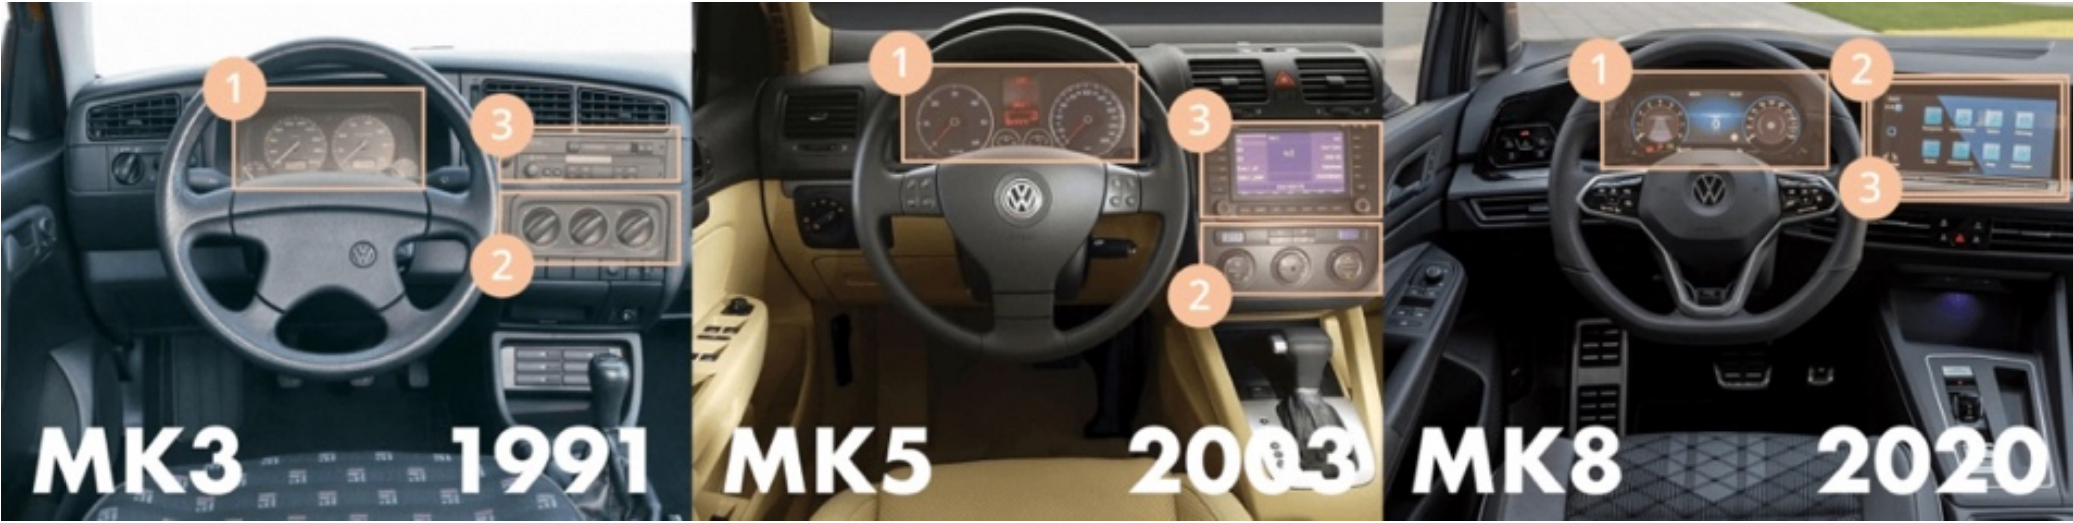
\includegraphics[width=0.9\textwidth]{evolutionTouchscreen.png}
    \caption{Evolución del panel en un Volkswagen Golf \cite{userExperience}.}
    \label{fig:imagen1}
\end{figure}

Esta adaptación es debido al ràpido avance tecnológico de los teléfonos móviles y tablets, la comodidad en la que se interactúa pulsando o deslizando sobre las pantallas de los dispositivos, es lo que ha promovido a los fabricantes de automóviles a incorporar las mismas características de las pantallas táctiles en el lugar de los controles físicos de los coches.  

\begin{figure}[h]
    \centering
    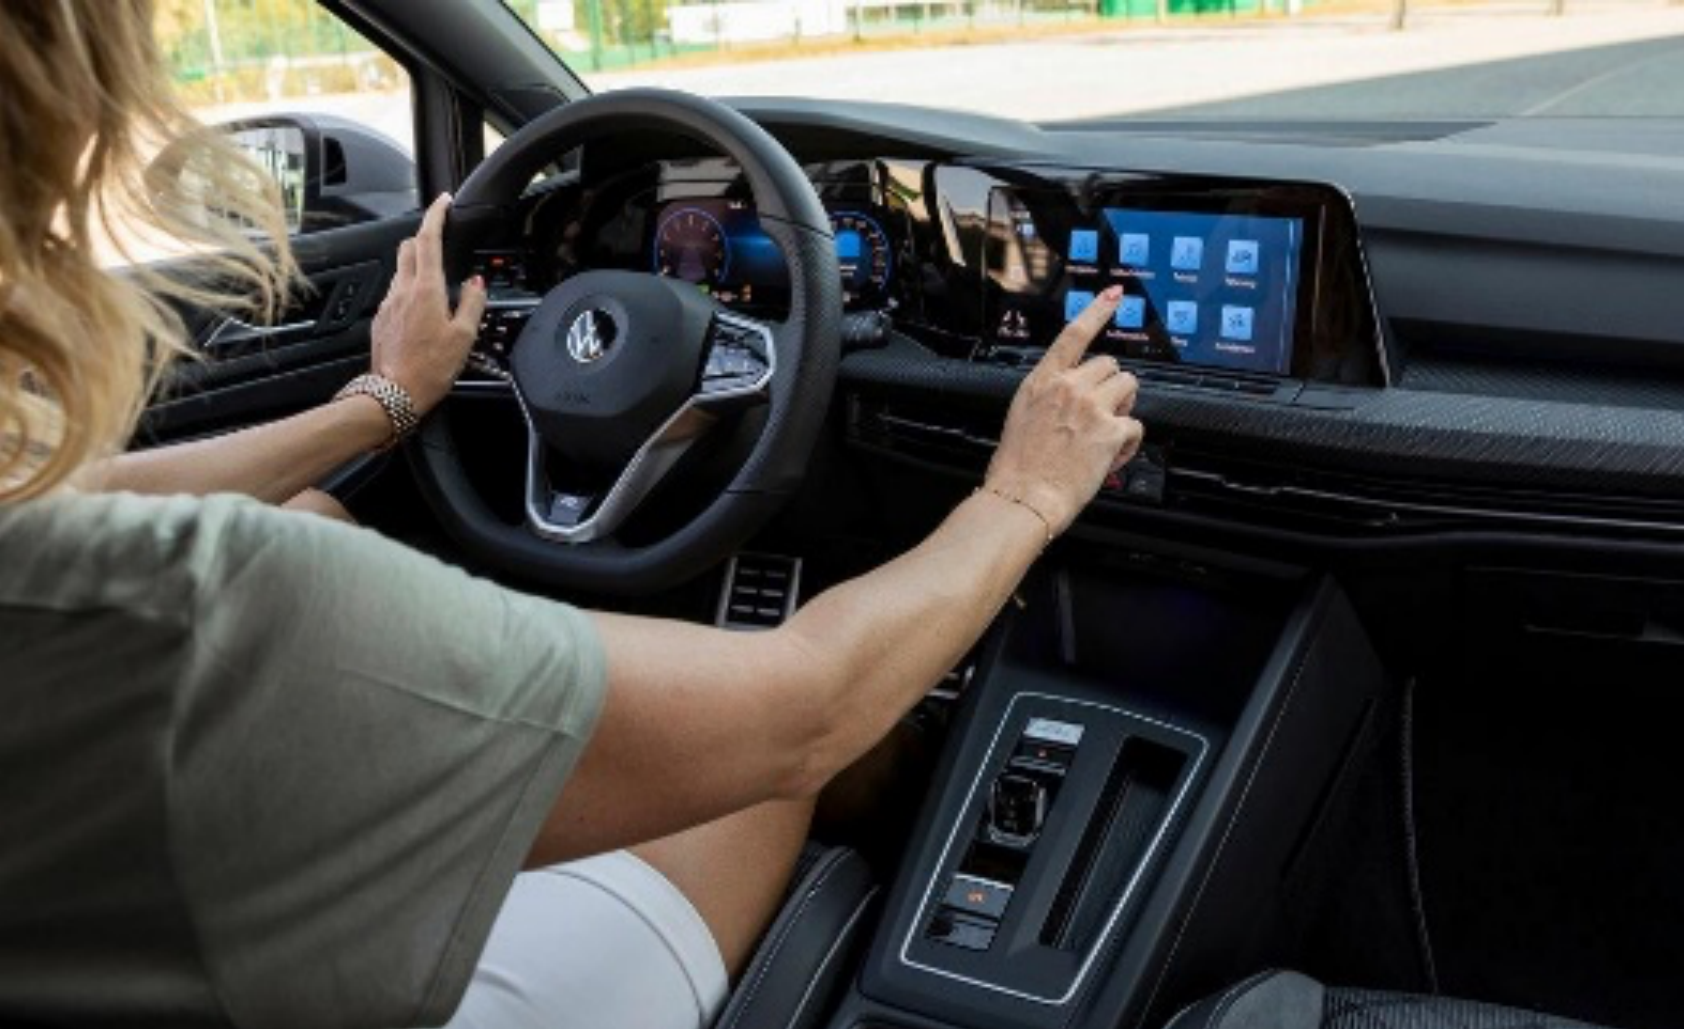
\includegraphics[width=0.7\textwidth]{usingTouchscreen.png}
    \caption{Conductor interaccionando con una pantalla táctil \cite{userExperience}.}
    \label{fig:imagen2}
\end{figure}

Las pantallas táctiles aportan bastantes beneficios, como pueden ser un diseño limpio y simplificado, siendo visualmente más atractivo al no contener tantos botones y diales, o flexibilidad y dinamicidad el la interfaz para añadir o mejorar funcionalidades.

Sin embargo, aunque permiten una interacción más sencilla y limpia, también presentan problemas de seguridad hacia el conductor. La distracción visual del conductor por la necesidad de desviar la vista de la carretera para interactuar con los paneles, lo que podría aumentar el riesgo de accidente o una falta de retroalimentación para las acciones que se realicen dificultaría al usuario manejar la pantalla sin mirar. Incluso en países como Reino Unido donde los vehículos tienen los volantes a la derecha, interaccionar con la pantalla con la mano izquierda podría ser difícil o incómodo. 

\subsection{Coches conectados}

El concepto de “coche conectado” surge de la integración de los coches en el Internet de las Cosas (IoT), al ser capaces de acceder a Internet, comunicarse con dispositivos inteligentes y recopilar datos en tiempo real. Inicialmente los automóviles contenían un número pequeño de Unidades de Control Electrónico (ECU), donde cada una era independiente de otra y realizaba una funcionalidad simple. Los coches de hoy en día pueden contener hasta 70 ECUs realizando muchas funcionalidades variadas, además de poder utilizar protocolos de comunicación que les permiten “hablar” con otros vehículos e infraestructuras, e incluso con Internet. Actualmente, incluso se ha logrado la integración de dispositivos móviles y smartphones en los paneles de los automóviles ofreciendo servicios avanzados de multimedia y entretenimiento. 
\cite{mobileIntegration}

\begin{figure}[h]
    \centering
    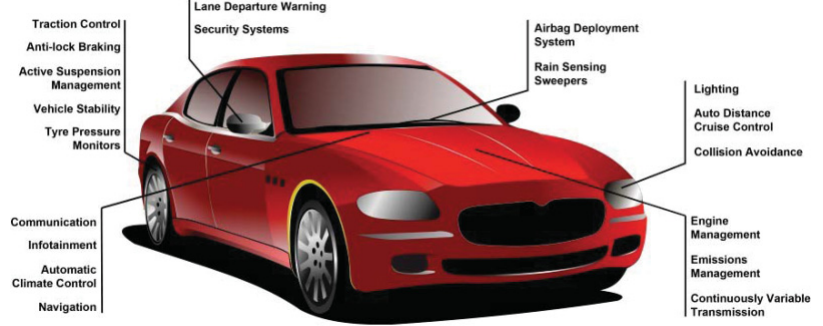
\includegraphics[width=0.9\textwidth]{ecu.png}
    \caption{Ejemplos de ECUs en un coche \cite{mobileIntegration}.}
    \label{fig:imagen3}
\end{figure}

\begin{figure}[H]
    \centering
    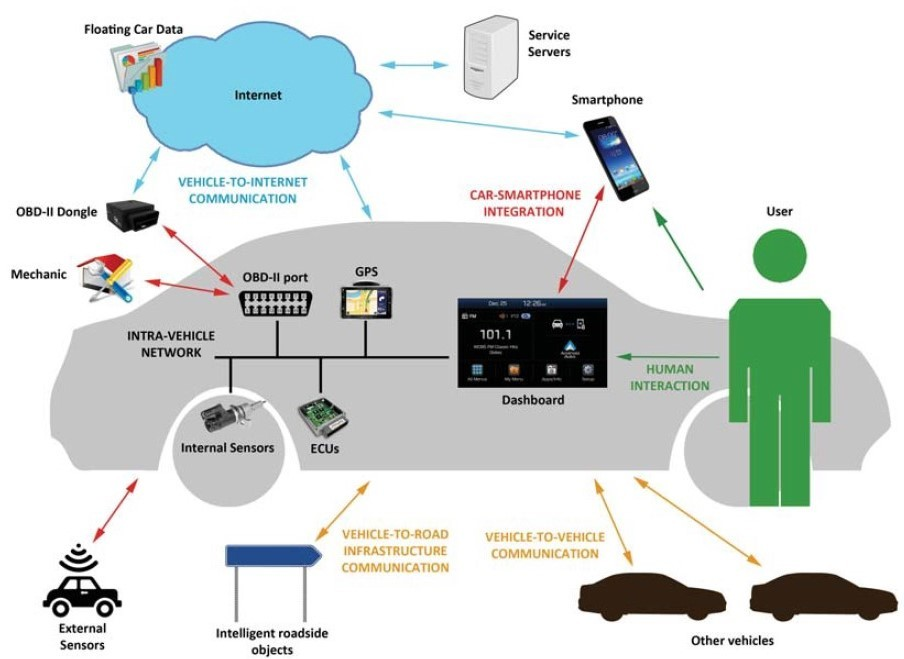
\includegraphics[width=0.9\textwidth]{connected_car_system.jpg}
	\caption{Visión general de un sistema de coche conectado \cite{mobileIntegration}.}
    \label{fig:imagen4}
\end{figure}

Al tener tantos dispositivos interconectados, las tecnologías y protocolos de comunicación en los coches conectados son fundamentales para su correcto funcionamiento, ya que permiten la interacción entre los componentes del vehículo, otros vehículos o las infraestructuras de las vías. Los diferentes tipos de comunicación que un coche conectado debe garantizar y las tecnologías disponibles para realizar dichas conexiones son las siguientes: 

\begin{itemize}

    \item \textbf{Vehicle To Sensors On Board communication (V2S) o Comunicación Intra-Vehicular:} esta comunicación se centra en la transmisión de información entre las ECUs y los sensores del vehículo, y se realiza mediante cables físicos o redes inalámbricas como Bluetooth o Ultra-Wideband. Un detalle a tener en cuenta es que aunque las redes inalámbricas ofrecen más versatilidad, presentan todavía problemas de seguridad y fiabilidad.
    \item \textbf{Vehicle To Vehicle Communication (V2V) o Comunicación Inter-Vehicular:} esta comunicación se centra en la transmisión de información entre diferentes coches sin la necesidad de un dispositivo remoto centralizado, utilizada principalmente para evitar accidentes, optimizar de rutas, compartir información multimedia y facilitar la interacción social entre conductores. Esta tecnología de comunicación enfrenta todavía desafíos ya una constante variación en la topología de la red o la presencia de obstáculos puede dificultar su gestión o interrupciones en el flujo de los datos.
    \item \textbf{Vehicle To Road Infrastructure Communication (V2R):} esta comunicación se centra en la transmisión de información entre un vehículo y una infraestructura de la vía compuesta por señales de tráfico, sensores de carretera y semáforos, y utilizada principalmente para una gestión eficiente del tráfico.
    \item \textbf{Vehicle To Internet Communication (V2I):} esta comunicación se centra en la transmisión de información entre un vehículo e Internet, utilizada principalmente para interaccionar con sus servicios y acceder a información multimedia. Se realiza mediante infraestructuras de red celular, al igual que un dispositivo móvil, utilizando una tarjeta SIM para permitir que el vehículo se conecte a una red 3G o 4G.

\end{itemize}

En cuanto a la integración de dispositivos móviles y smartphones con los coches conectados, se han desarrollado soluciones software capaces de permitir a la pantalla del coche acceder a los datos del dispositivo, e incluso permite al usuario controlar aplicaciones del dispositivo en la pantalla. Esta integración ofrece varias ventajas, como pueden ser una personalización diferente para cada usuario que depende de cada dispositivo, o además facilitar a los desarrolladores de aplicaciones crear aplicaciones sobre una plataforma genérica en vez de un modelo de pantalla específico. Las soluciones de integración más extendidas son: 

\begin{itemize}

    \item \textbf{MirrorLink:} desarrollado por el Car Connectivity Consortium (CCC), y permite la conexión mediante USB o Wi-Fi Direct. Crea directrices para la interfaz gráfica de las aplicaciones, con iconos de gran tamaño facilitando una navegación rápida y sencilla.
    \item \textbf{Applink:} desarrollada por Ford, y permite realizar distintas acciones dentro del vehículo como mostrar mensajes en la pantalla, reproducir música y ofrecer controles por voz.
    \item \textbf{Apple CarPlay:} solución desarrollada para dispositivos iPhone, extendiendo las funcionalidades del sistema estándar del vehículo, y permite controlar aplicaciones mediante la pantalla, comandos de voz con SIRI, y llamadas y mensajes con manos libres.
    \item \textbf{Android Auto:} solución desarrollada por la Open Automotive Alliance, y centrada en la conexión con dispositivos Android. Proporciona un tablero simple que permite el acceso a sistemas de navegación, como por ejemplo Google Maps, además de música, llamadas telefónicas, comandos de voz, etc.

\end{itemize}

\begin{figure}[h]
	\centering
	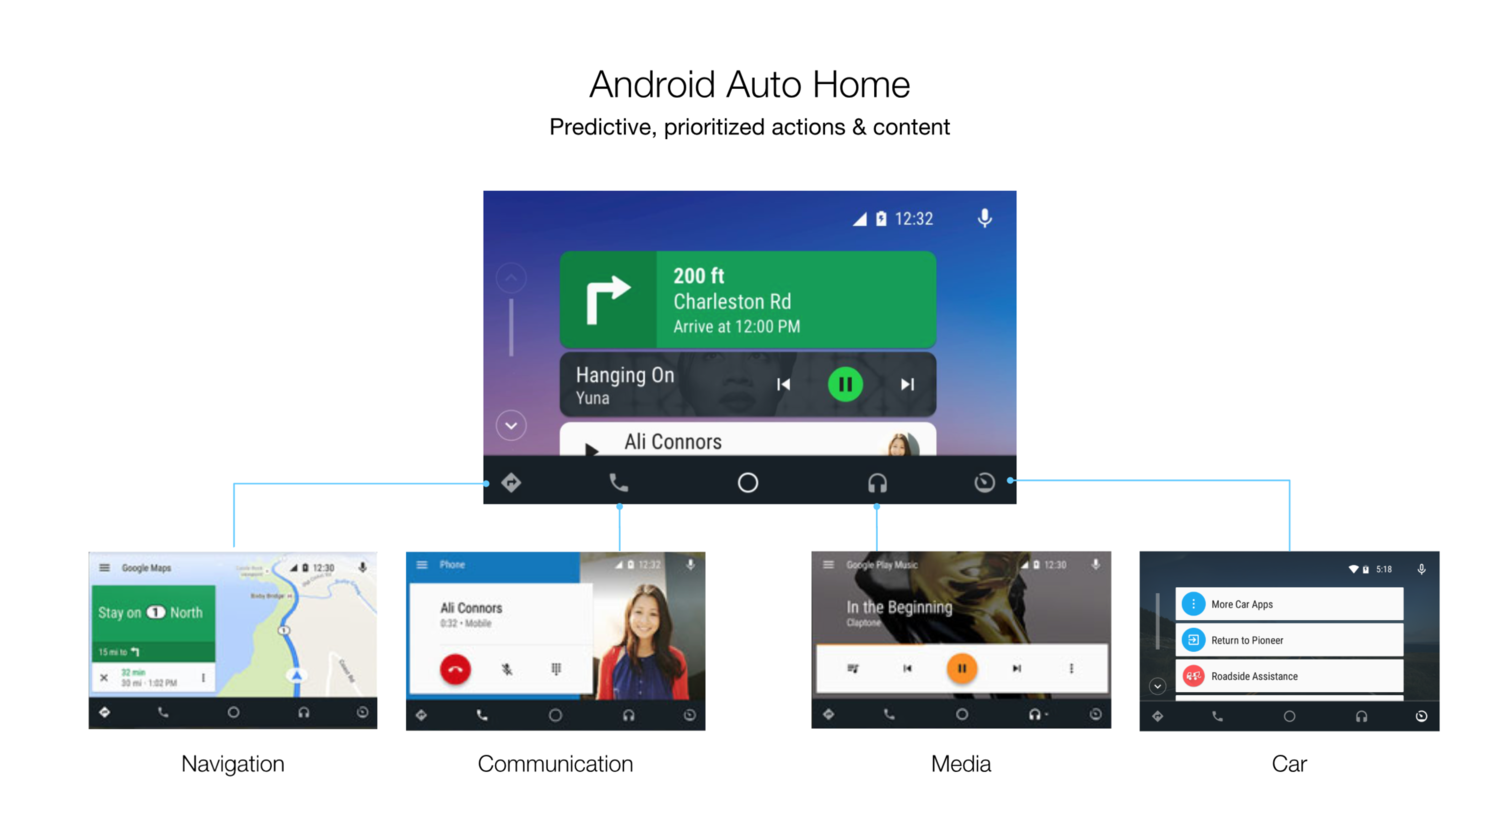
\includegraphics[width=0.7\textwidth]{androidAuto.png}
	\caption{Ejemplos de interfaces de Android Auto en la pantalla del coche.}
	\label{fig:imagen5}
\end{figure}

Actualmente, de las tecnologías anteriores las más populares y mayoritariamente implementadas  son las dos últimas,  Apple CarPlay y Android Auto, debido a que tienen un mayor número de funcionalidades y tienen un mayor número de dispositivos con dicho sistema operativo compatible.

\begin{figure}[H]
    \centering
    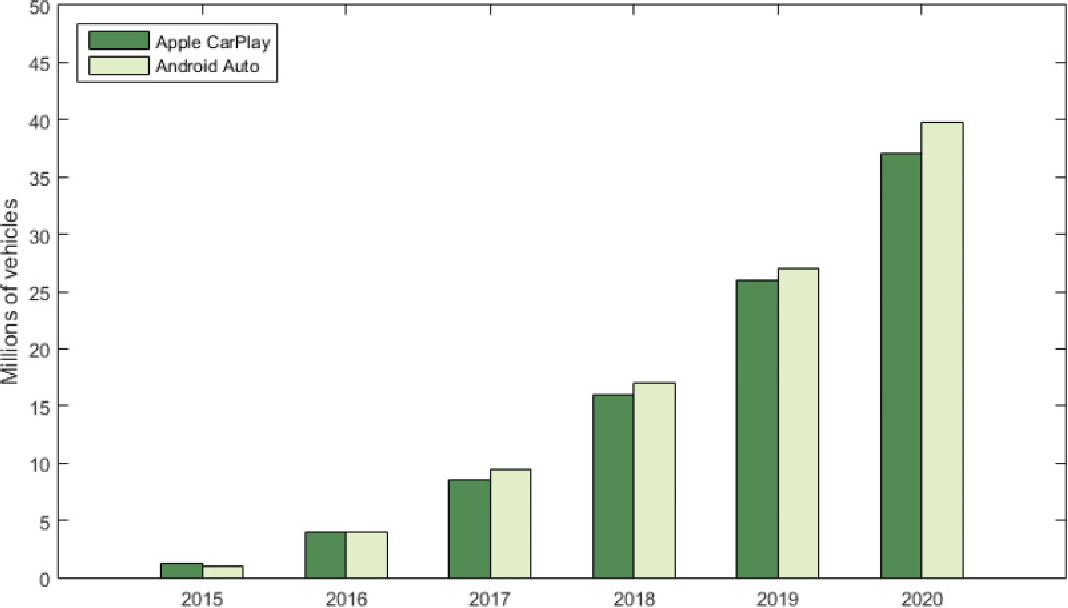
\includegraphics[width=0.7\textwidth]{integrationSolution.png}
	\caption{Ventas de coches con Apple CarPlay vs Android Auto \cite{mobileIntegration}.}
	\label{fig:imagen6}
\end{figure}

\subsection{Heads Up Display (HUD)}

Los sistemas Head-Up Display (HUD) fueron desarrollados originalmente para aviadores durante la Primera Guerra Mundial, los cuales servían para percibir aviones enemigos, y que posteriormente fueron evolucionando para mostrar más información como altitud, velocidad del viento, indicador de horizonte, etc. Actualmente se han introducido también en vehículos a tierra, los coches, mostrando datos esenciales sobre el parabrisas del vehículo.
\cite{hudPaper}

\begin{figure}[h]
    \centering
    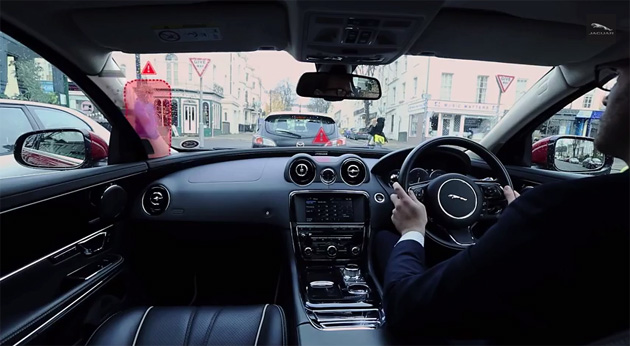
\includegraphics[width=0.7\textwidth]{hud.png}
    \caption{Vista de un HUD de un Jaguar \cite{hudPaper}.}
    \label{fig:imagen7}
\end{figure}

La estructura de un HUD se compone de tres componentes: el combinador, la superficie donde se proyecta la imagen; el proyector, el componente que genera y dirige la imagen hacia el combinador; y la unidad de procesamiento, que gestiona los datos obtenidos y controla la protección.

\begin{figure}[h]
    \centering
    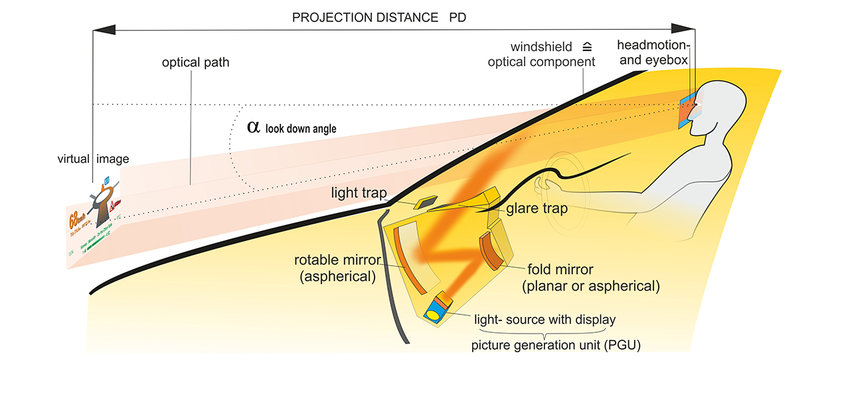
\includegraphics[width=0.7\textwidth]{hudWork.png}
    \caption{Funcionamiento y componentes de un HUD \cite{hudPaper}.}
    \label{fig:imagen8}
\end{figure}

La información que es proporcionada por un HUD de un automóvil está centrada en información relacionada con la conducción y el estado del vehículo: características de la carretera como límites de velocidad y condiciones del camino, o navegación con mapas y direcciones. Todo esto es útil para mantener al conductor informado, y proporcionar advertencias en caso de eventos peligrosos que puedan incurrir a la seguridad.

También se han desarrollado dispositivos HUD comerciales, que pueden instalarse de manera externa, aunque tienen limitaciones para usar la información de navegación al no ser integrados. 

Algunos vehículos modernos incluyen incluso funcionalidades como visión nocturna, mediante el uso de cámaras infrarrojas para mejorar la visibilidad en condiciones de poca luz, y proyectando esa información en el HUD. 

\begin{figure}[h]
    \centering
    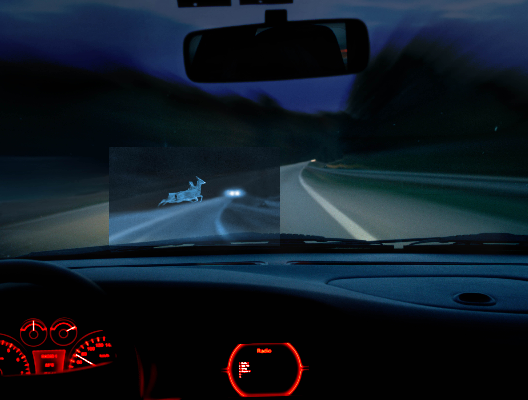
\includegraphics[width=0.5\textwidth]{nigthHUD.png}
    \caption{Visión de cámara de infrarrojos en el HUD \cite{hudPaper}.}
    \label{fig:imagen9}
\end{figure}

También existen casos experimentales donde se implementan en los espejos retrovisores para proporcionar información de vistas traseras. 

\begin{figure}[H]
    \centering
    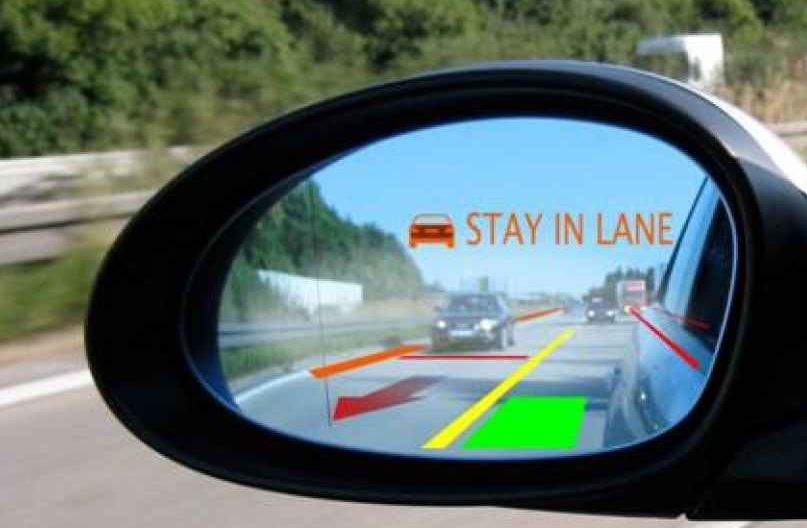
\includegraphics[width=0.5\textwidth]{retroHUD.png}
    \caption{Visión de HUD en espejos retrovisores \cite{hudPaper}.}
    \label{fig:imagen10}
\end{figure}

\section{Sistemas Avanzados de Ayuda a la Conducción (ADAS)}

Los Sistemas Avanzados de Asistencia al Conductor son un conjunto de tecnologías, combinando hardware y software, que ayudan a tener una conducción segura y eficiente. El objetivo principal es reducir el riesgo de accidentes y mejorar la experiencia de conducción mediante el uso de sensores, cámaras, radares y distintos dispositivos que monitorean el entorno alrededor del vehículo y avisan de manera activa al conductor. De esta manera, no sólo mejoran la seguridad de los ocupantes de un vehículo, también proporcionan más seguridad a otros ocupantes de las vías como pueden ser los peatones o ciclistas.
\cite{adasDGT}

Debido a la importancia y eficacia de estos sistemas para la seguridad, la Unión Europea aprobó en 2019 el Nuevo Reglamento de Seguridad 2019/2144 \cite{adasDGT} que recogía una serie de requisitos a cumplir para garantizar la seguridad de los vehículos y las personas. En España se implantó el 6 de julio de 2022 dicho Reglamento, y obliga a todos los coches nuevos de fábrica a incorporar al menos los siguientes ocho sistemas ADAS: 

\begin{itemize}

    \item \textbf{Detector de Fatiga y Somnolencia (DDR):} este sistema de ADAS se enfoca a prevenir distracciones del conductor debido a somnolencia, cansancio o falta de atención. Utiliza distintos tipos de tecnologías como: sensores en el volante para analizar la presión que se ejerce sobre el o la brusquedad de las correcciones de dirección; una cámara de reconocimiento facial que detecta el exceso de parpadeo o la visión de la mirada; o temporizador en el motor que recoge el tiempo que lleva en marcha. Si el sistema detecta anomalías o un tiempo de marcha largo, emite una señal o texto por los paneles del coche para avisar al conductor.
    \begin{figure}[H]
		\centering
		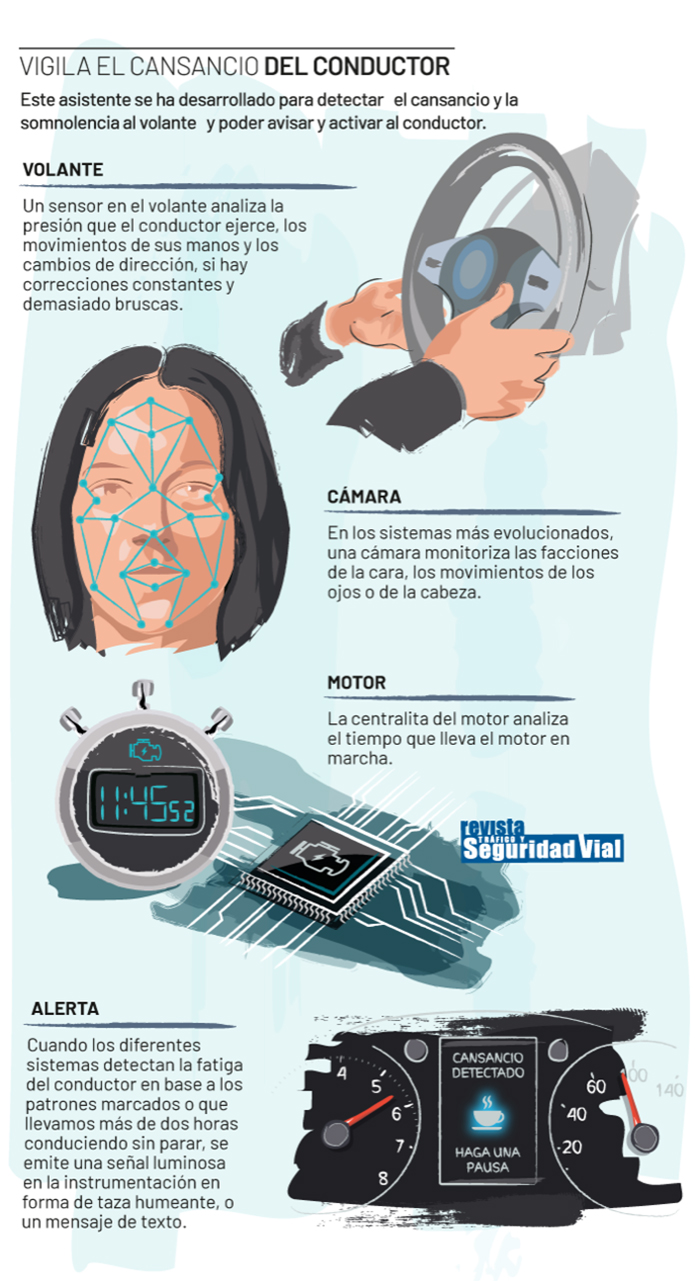
\includegraphics[width=0.6\textwidth]{adasDDR.jpg}
		\caption{Funcionamiento del sistema DDR \cite{adasObligatorios}.}
		\label{fig:imagen11}
	\end{figure}
	\item \textbf{Asistente de velocidad inteligente (ISA):} este sistema ADAS se enfoca en limitar la velocidad máxima a la que se circula mediante una cámara interior que lee las senales de las vías. La velocidad permitida es mostrada en el cuadro de mando del conductor, y el software actúa sobre el motor o el acelerador impidiendo que supere esa velocidad máxima, aunque se puede desconectar mediante un botón o pisando con fuerza el acelerador.
    \begin{figure}[H]
		\centering
		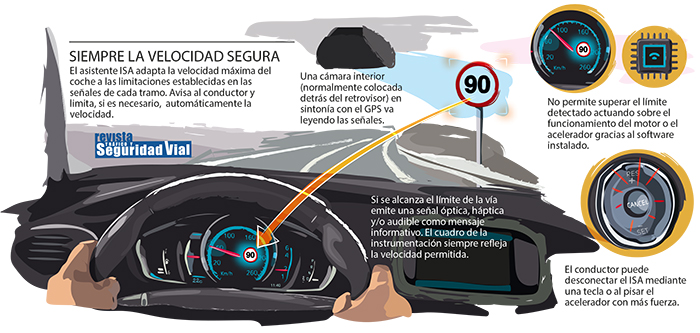
\includegraphics[width=0.8\textwidth]{adasISA.jpg}
		\caption{Funcionamiento del sistema ISA \cite{adasObligatorios}.}
		\label{fig:imagen12}
	\end{figure}
	\item \textbf{Cámara Trasera con Detección de Tráfico Cruzado (RCTA):} este sistema ADAS se enfoca en facilitar la visión del conductor en la marcha atrás con cámaras que muestran la imagen en el panel. También detecta posibles obstáculos que puedan estar en la trayectoria de la maniobra, advierte al conductor en la pantalla o en el retrovisor, y si el conductor no reacciona puede llegar a detener el coche de manera automática.
    \begin{figure}[H]
		\centering
		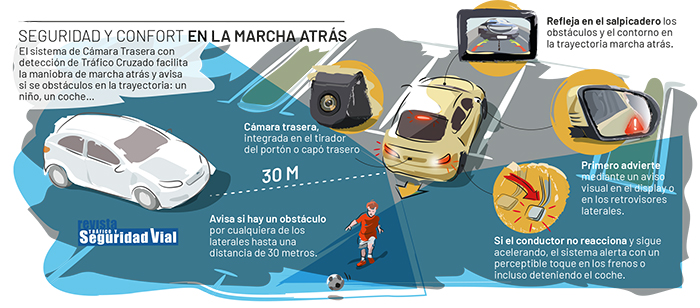
\includegraphics[width=0.8\textwidth]{adasRCTS.jpg}
		\caption{Funcionamiento del sistema RCTA \cite{adasObligatorios}.}
		\label{fig:imagen13}
	\end{figure}
	\item \textbf{Caja negra (EDR):} este sistema ADAS se enfoca en recopilar información, en caso de accidente, de los momentos anteriores y posteriores a él, para poder evaluar las posibles causas y estado de los sistemas del vehículo. El EDR está ubicado debajo del asiento del conductor, del tamaño aproximado de un teléfono móvil, y se puede conectar a un ordenador para obtener la información necesaria.
    \begin{figure}[H]
		\centering
		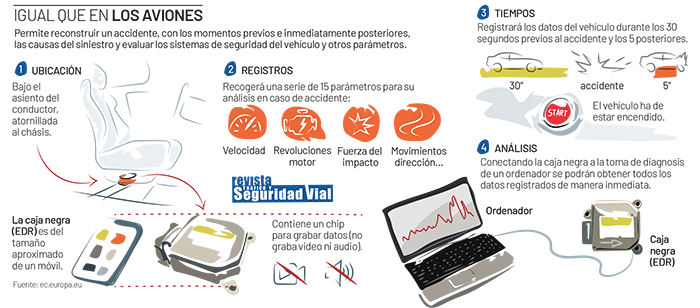
\includegraphics[width=0.7\textwidth]{adasEDR.jpg}
		\caption{Funcionamiento del sistema EDR \cite{adasObligatorios}.}
		\label{fig:imagen14}
	\end{figure}
	\item \textbf{Alerta de cambio involuntario de carril (LDW):} este sistema ADAS se enfoca en controlar que el vehículo no se desvía del carril por el que circula por una posible falta de atención del conductor. Utiliza una cámara frontal que detecta de forma continua las líneas del carril por el que circula, y en caso de que no se haya activado ningún intermitente y el vehículo esté saliendo del carril, avisa mediante una señal en el cuadro, un sonido o vibraciones. Además, si dispone de algún sistema de mantenimiento de carril, podría activarse para mantener el vehículo correctamente en el carril.
    \begin{figure}[H]
		\centering
		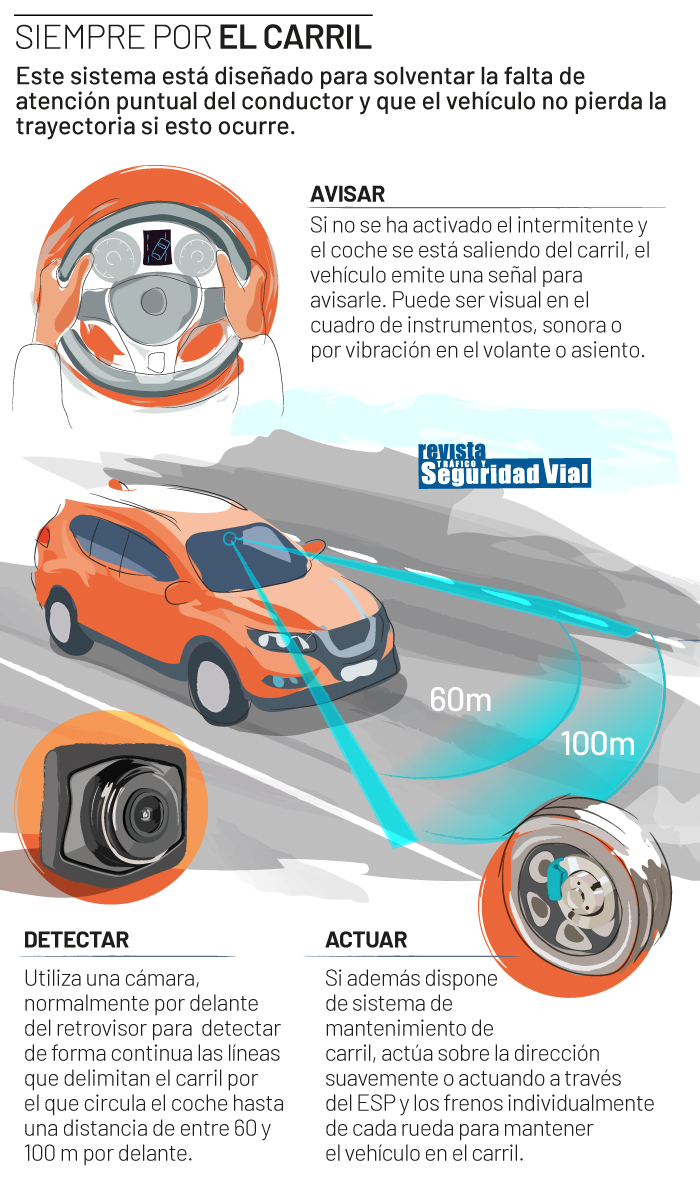
\includegraphics[width=0.5\textwidth]{adasLDW.jpg}
		\caption{Funcionamiento del sistema LDW \cite{adasObligatorios}.}
		\label{fig:imagen15}
	\end{figure}
	\item \textbf{Sistema de frenada de emergencia (BAS y EBA):} este sistema ADAS se enfoca en reducir el riesgo de colisión por alcance. Al realizar una frenada brusca, detecta si la intensidad con la que se pisa es la adecuada, y si no es suficiente el sistema interacciona frenando a la máxima intensidad posible. Además dispone de distintos sensores que permite distinguir a las personas y realiza un aviso, si el conductor no reacciona al aviso se activa el freno de manera automática.
    \begin{figure}[H]
		\centering
		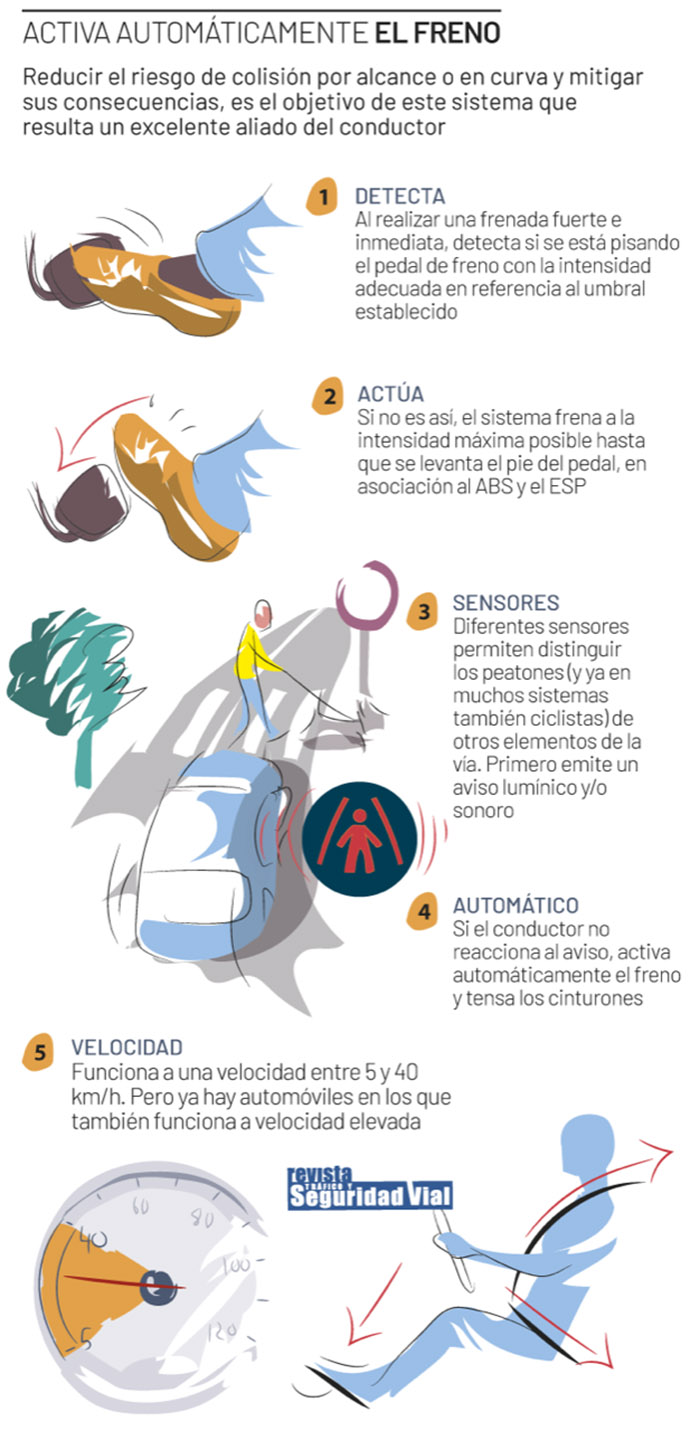
\includegraphics[width=0.6\textwidth]{adasBASyEBA.jpg}
		\caption{Funcionamiento del sistema BAS y EBA \cite{adasObligatorios}.}
		\label{fig:imagen16}
	\end{figure}
	\item \textbf{Bloqueo de vehículo con alcoholímetro (Alcolock):} este sistema ADAS se enfoca en el control de la conducción tras la ingesta de alcohol. El vehículo dispone de un sistema de alcoholímetro, conectado al motor de arranque, y que impedirá al conductor arrancar el motor si la tasa de alcohol analizada por la boquilla sea superior al índice permitido. El sistema tendrá implementado sensores con tecnologías de reconocimiento de huellas dactilares, detección facial o fotografías digitales, que serán guardadas en memoria al igual que el historial de análisis, que servirá para identificar al usuario e impedir la falsificación o el fraude.
    \begin{figure}[H]
		\centering
		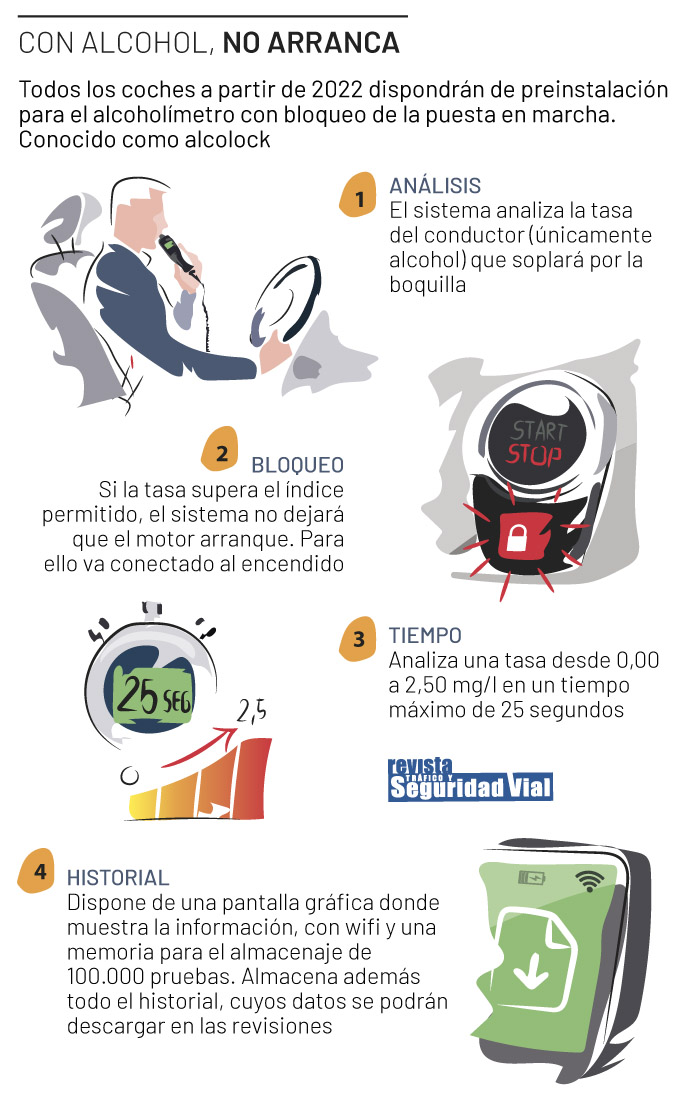
\includegraphics[width=0.8\textwidth]{adasAlcolock.jpg}
		\caption{Funcionamiento del sistema Alcolock \cite{adasObligatorios}.}
		\label{fig:imagen17}
	\end{figure}
	\item \textbf{Alerta de cinturón en las plazas traseras:} este sistema ADAS se enfoca en controlar y avisar el uso correcto del cinturón de seguridad en las plazas traseras. El sistema determina mediante un sensor de carga si la plaza está ocupada, y mediante un sensor de la hebilla si está bien cerrado. En caso de que el vehículo recorra una determinada distancia, un determinado tiempo o supere los 25 km/h y no se haya puesto el cinturón de una manera correcta, el sistema avisa automáticamente mediante señales visuales y acústicas.
	\begin{figure}[H]
		\centering
		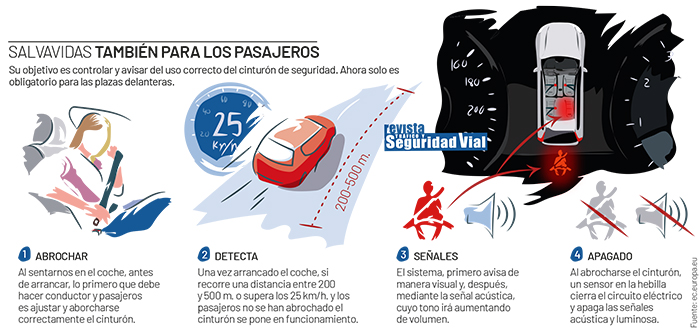
\includegraphics[width=0.8\textwidth]{adasCinturon.jpg}
		\caption{Funcionamiento del sistema de Alerta de cinturón en las plazas traseras \cite{adasObligatorios}.}
		\label{fig:imagen18}
	\end{figure}

\end{itemize}

\section{Vehículos Autónomos}

El gran avance de la tecnología, en el ámbito del IoT y los sistemas embebidos, hacen que los vehículos se vuelvan cada vez más inteligentes, hasta llegar al punto de poder realizar acciones de forma autónoma sin intervención de las personas. Los vehículos autónomos (AV) tienen como objetivo mejorar la seguridad en las vías, facilitar las maniobras diarias de los conductores y disminuir el riesgo de accidentes debido a cansancio o fatiga, y optimizar recursos y tiempo de manera eficiente.
\cite{autonomousVehicles2}

Un vehículo autónomo puede clasificarse en diferentes niveles de autonomía, dependiendo del grado o acciones que llega a realizar el vehículo de forma autónoma en comparación con el conductor. Existe una normativa estandarizada, definida por la Sociedad de Ingenieros Automotrices (SAE), el estándar J3016 o Taxonomy and Definitions for Terms Related to On-Road Motor Vehicle Automated Driving Systems \cite{sae}, en el que se describe seis niveles de autonomía 
\cite{autonomousVehicles}:

\begin{figure}[H]
	\centering
	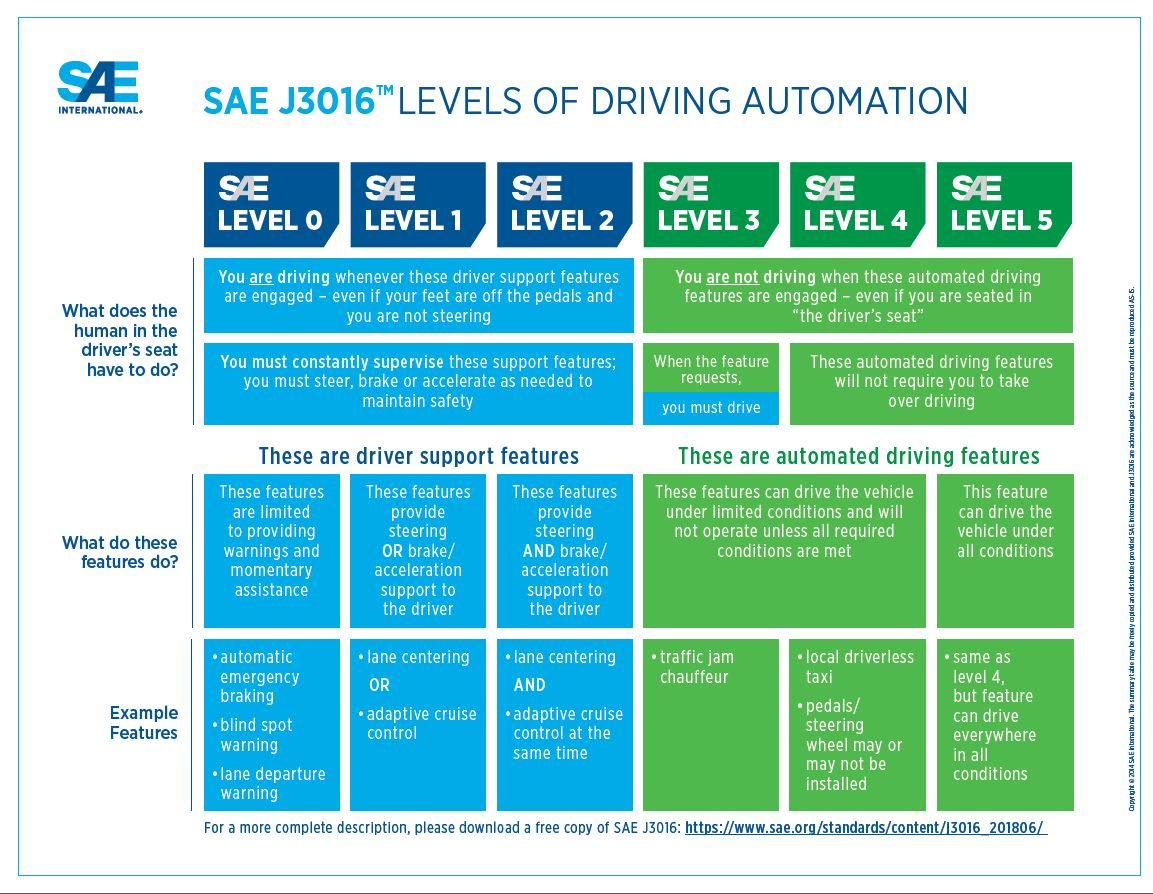
\includegraphics[width=\textwidth]{saeLevels.jpg}
	\caption{Niveles de autonomía según el estándar SAE J3016 \cite{autonomousVehicles}.}
	\label{fig:imagen19}
\end{figure}

\begin{itemize}

    \item \textbf{SAE Nivel 0 (Sin Automatización):} en este nivel, el conductor es responsable de todas las acciones relacionadas a la conducción, como son la aceleración, el frenado, el manejo de dirección y el uso de señales. El vehículo puede tener instalado sistemas de advertencia, como alertas de colisión o de objetos en punto ciego, pero en ningún caso realiza alguna acción controlando el vehículo por el conductor.
    \item \textbf{SAE Nivel 1 (Asistencia al Conductor):} en este nivel, se dispone de sistemas que pueden controlar funciones específicas del vehículo, como la aceleración (control de crucero adaptativo), el frenado (frenado de emergencia) o el manejo de direccion (sistema de mantenimiento de carril). El conductor debe estar atento y en supervisión constante para tomar el control de vuelta de los pedales en caso de necesidad.
    \item \textbf{SAE Nivel 2 (Automatización Parcial):} en este nivel, el vehículo puede además controlar la dirección de forma autónoma y simultánea con la aceleración y el frenado, pero el conductor debe estar al igual en supervisión constante sobre el entorno y tomar el control en caso necesario.
    \item \textbf{SAE Nivel 3 (Automatización Condicional):} en este nivel, el vehículo es capaz de percibir el estado del entorno de manera autónoma, y controlar todas las funciones de conducción en determinadas condiciones simples, como en autopistas. Aun así, en este caso el conductor debe estar en supervisión para tomar el control si el sistema lo solicita.
    \item \textbf{SAE Nivel 4 (Alta Automatización):} en este nivel, el vehículo puede encargarse de todas las funciones de forma autónoma en situaciones específicas y bien definidas, como por ejemplo en autopistas o áreas urbanas. El conductor sigue necesitando tener presencia en determinadas circunstancias, pero en este nivel ya existe la posibilidad de no utilizar volante ni pedales.
    \item \textbf{SAE Nivel 5 (Automatización Completa):} en este nivel, el vehículo es capaz de encargarse de todas la funciones en cualquier situación sin la necesidad de presencia humana.

\end{itemize}

Los vehículos autónomos están equipados con una gran cantidad de sensores y sistemas que les permiten lograr la percepción del entorno y poder conducir de una manera segura 
\cite{autonomousVehicles}:

\begin{figure}[h]
	\centering
	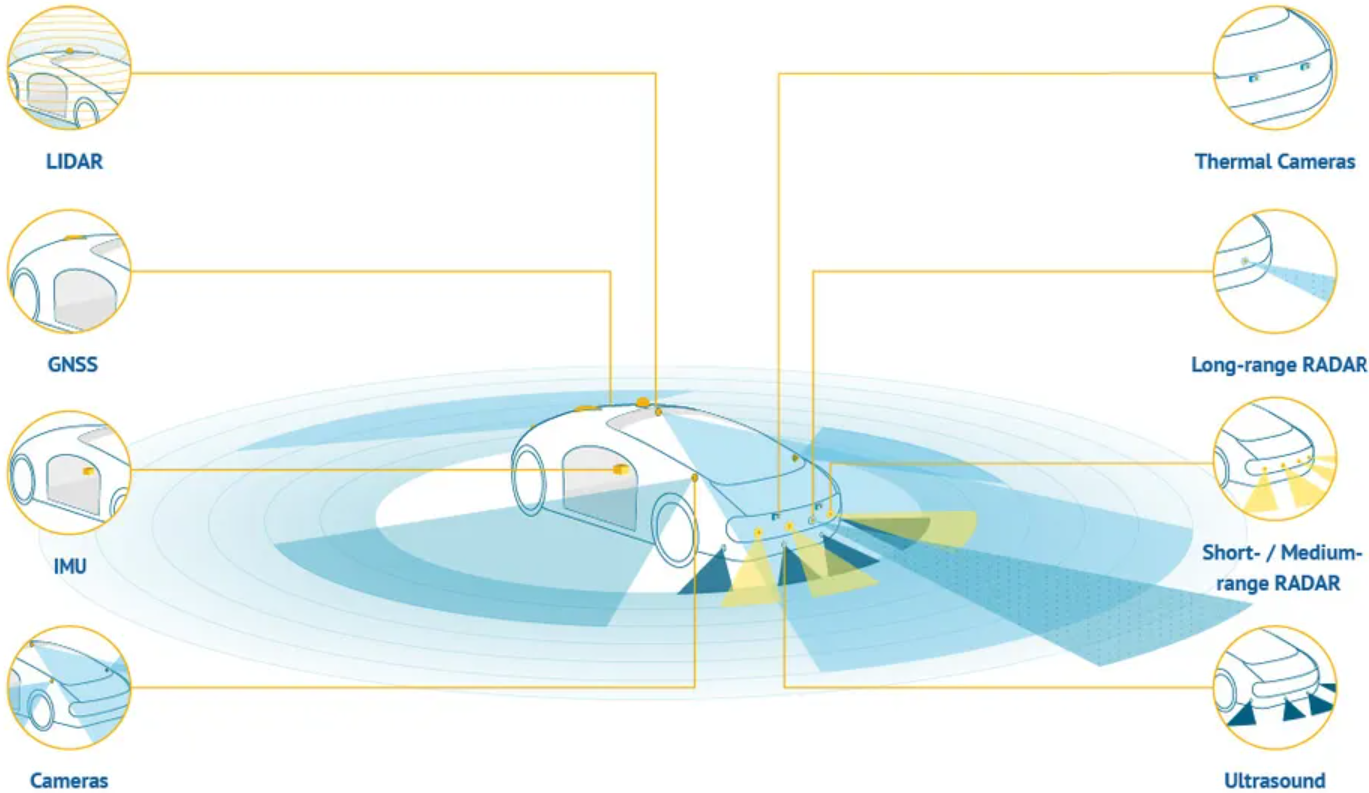
\includegraphics[width=0.9\textwidth]{saeSensors.png}
	\caption{Sensores en un vehículo autónomo \cite{autonomousVehicles}.}
	\label{fig:imagen20}
\end{figure}

\begin{itemize}

    \item \textbf{Light Detection and Ranging (LIDAR):} sensor que funciona mediante detección láser, analizando la luz reflejada que se envía. Este sensor es capaz de detectar los objetos de alrededor del vehículo y crear mapas virtuales de 2D o 3D.
    \item \textbf{Radio Detection and Ranging (RADAR):} sensor que funciona mediante ondas electromagnéticas que detectan los obstáculos o vehículos cercanos. Pueden ser de largo alcance, medio alcance o corto alcance, y se usan en sistemas como el control de crucero adaptativo, la advertencia de colisión o la detección del ángulo muerto.
    \item \textbf{Global Navigation Satellite System (GNSS):} conjunto de sistemas que funcionan mediante señal de los satélites, como por ejemplo el GPS, y proporciona información precisa sobre la ubicación y la hora.
    \item \textbf{Sensores Ultrasónicos:} sensores que detectan objetos en una distancia muy cercana al vehículo, utilizados en sistemas de asistencia al estacionamiento.
    \item \textbf{Unidad de Medición Inercial (IMU):} sensor que mide el movimiento lineal y angular del vehículo utilizando acelerómetros y giroscopios. La información que recibe se combina con los datos del sistema GPS para obtener una mayor precisión en la posición.
    \item \textbf{Cámaras térmicas:} cámaras que detectan el calor, con un rango más amplio que los faros, y son útiles para la detección de obstáculos, ya sean personas, animales u otros coches, en condiciones difícilmente perceptibles, como por la noche, en zona de humo o con un brillo solar intenso.
    \item \textbf{Cámaras de video:} cámaras de alta resolución, que monitorean y transmiten de manera constante imágenes de la vía, usadas para procesar información relevante como señales de tráfico, peatones o ciclistas.

\end{itemize}

El conjunto de sensores, junto a los sistemas ADAS, son lo que permiten a los conductores circular de manera más segura, y lo que hace posible que los vehículos autónomos puedan realizar tareas de conducción sin la intervención del conductor.

\begin{figure}[h]
	\centering
	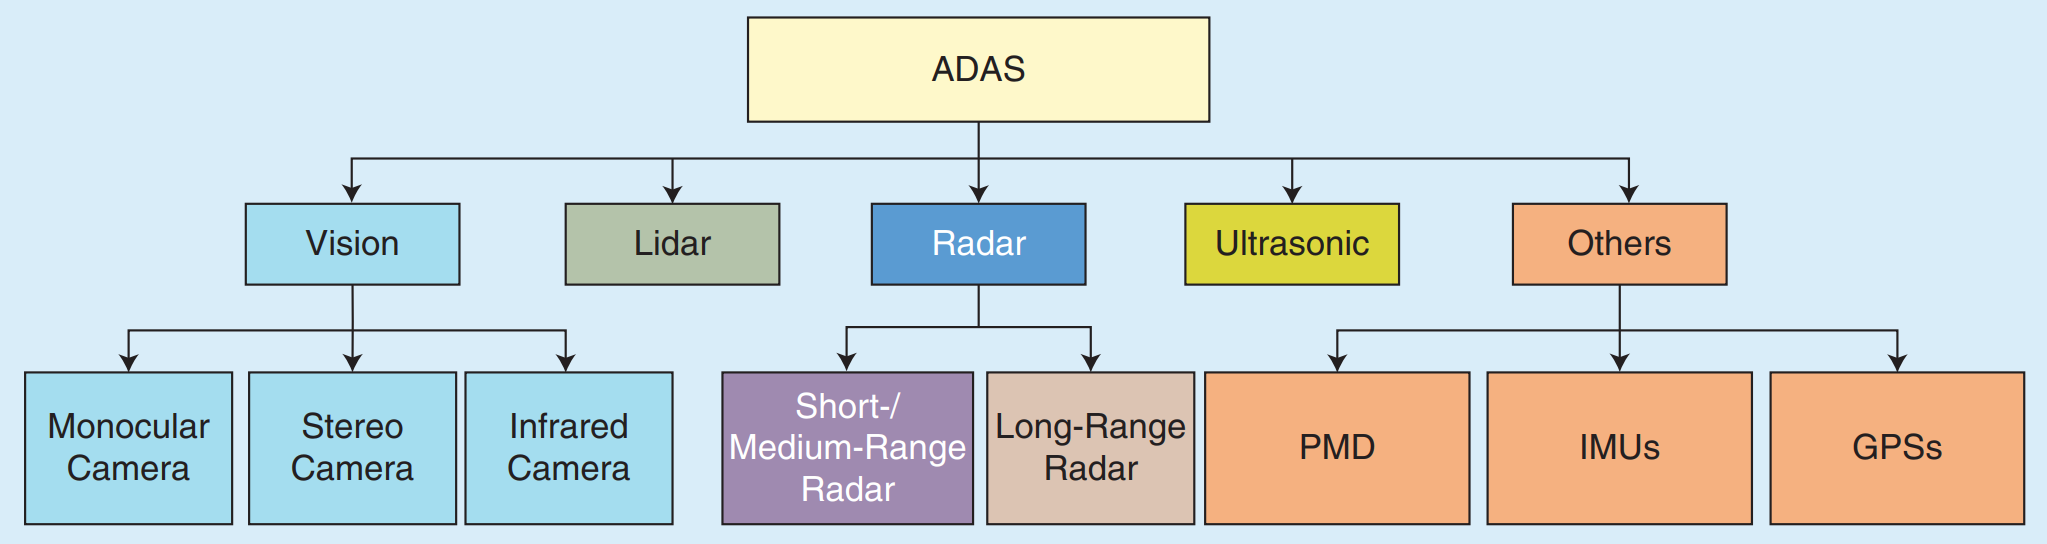
\includegraphics[width=0.9\textwidth]{adasSensorWorkflow.png}
	\caption{Clasificación de sensores usados en sistemas ADAS \cite{adasSensors}.}
	\label{fig:imagen21}
\end{figure}

\begin{figure}[h]
	\centering
	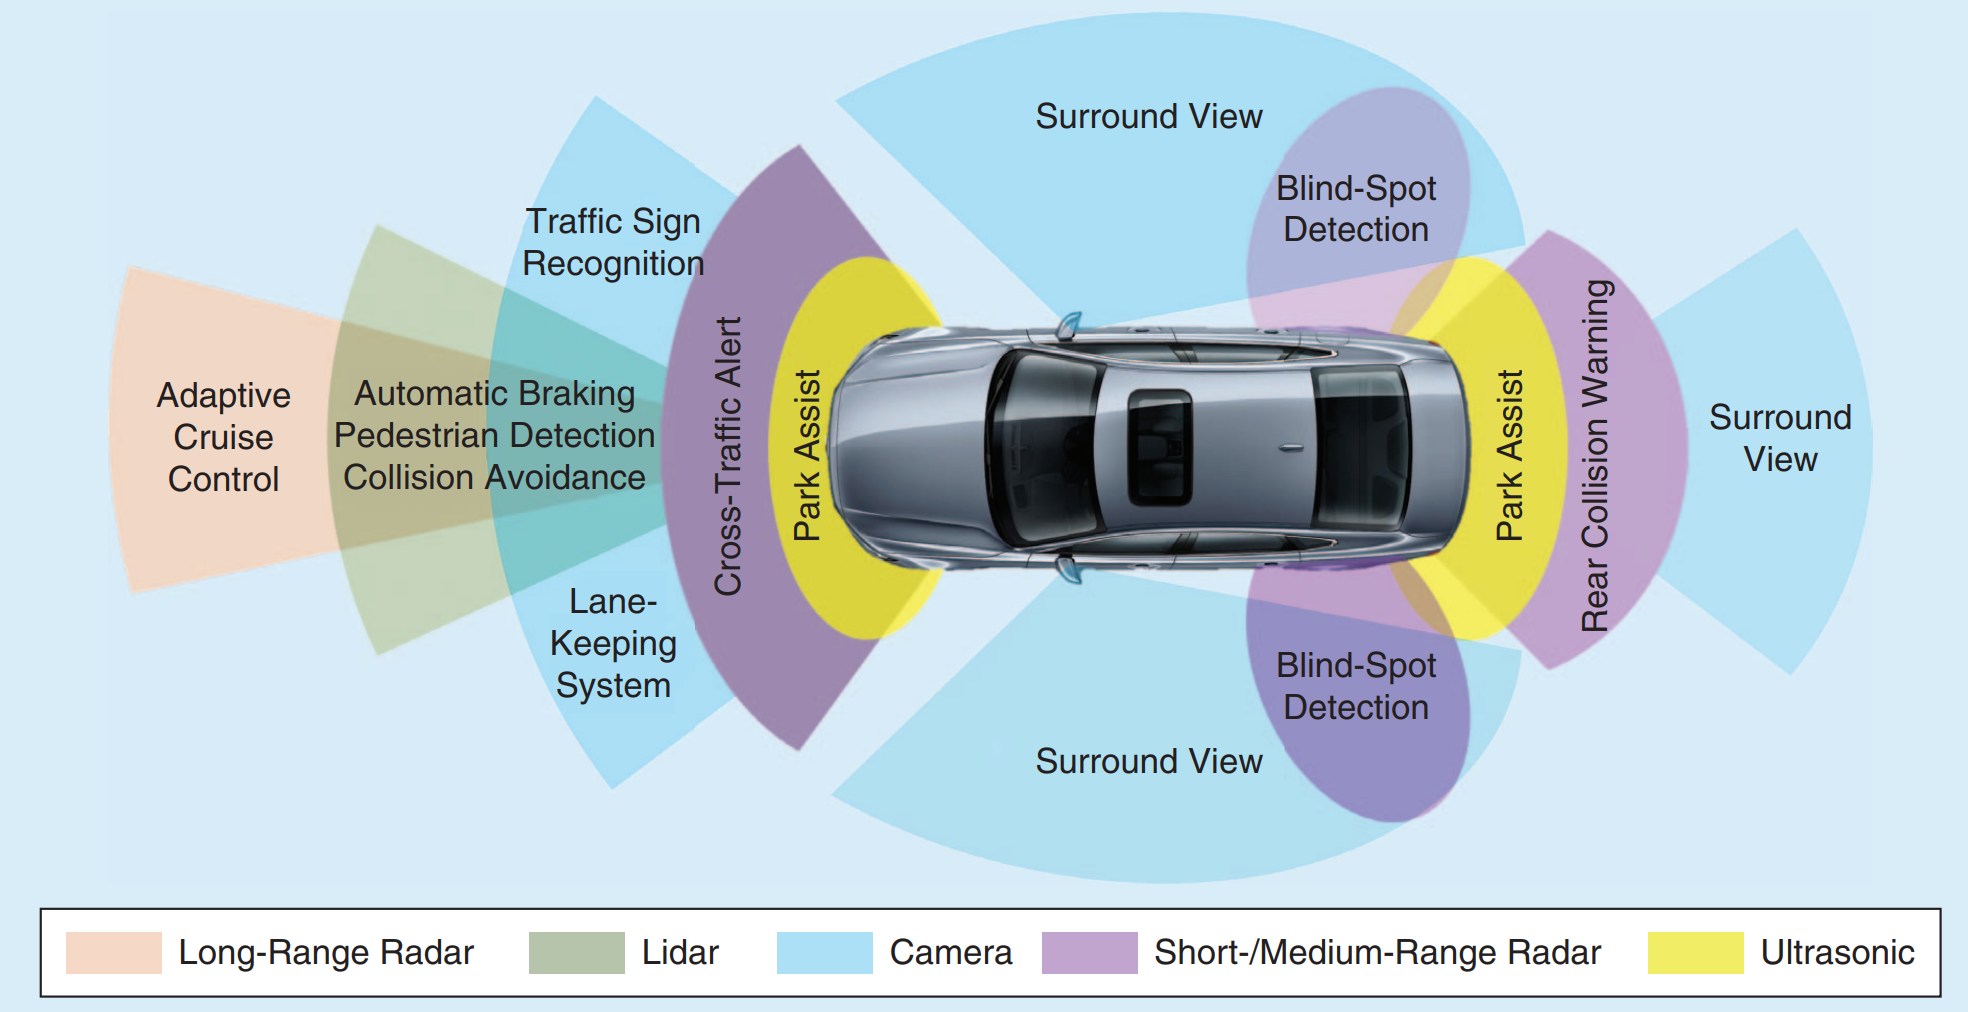
\includegraphics[width=0.9\textwidth]{adasSensorRange.png}
	\caption{Rangos sobre los que actúan los sensores \cite{adasSensors}.}
	\label{fig:imagen22}
\end{figure}

\section{Inteligencia Artificial y Aprendizaje Automático}

La Inteligencia Artificial (IA) se define como “capacidad de las máquinas para imitar la inteligencia de las personas humanas en la realización de tareas” \cite{deepLearning}. La investigación en IA está centrada en el desarrollo de dispositivos que perciben su entorno, resuelven problemas, y aprenden de los errores que sirvan posteriormente, para alcanzar un objetivo específico.

\begin{figure}[h]
	\centering
	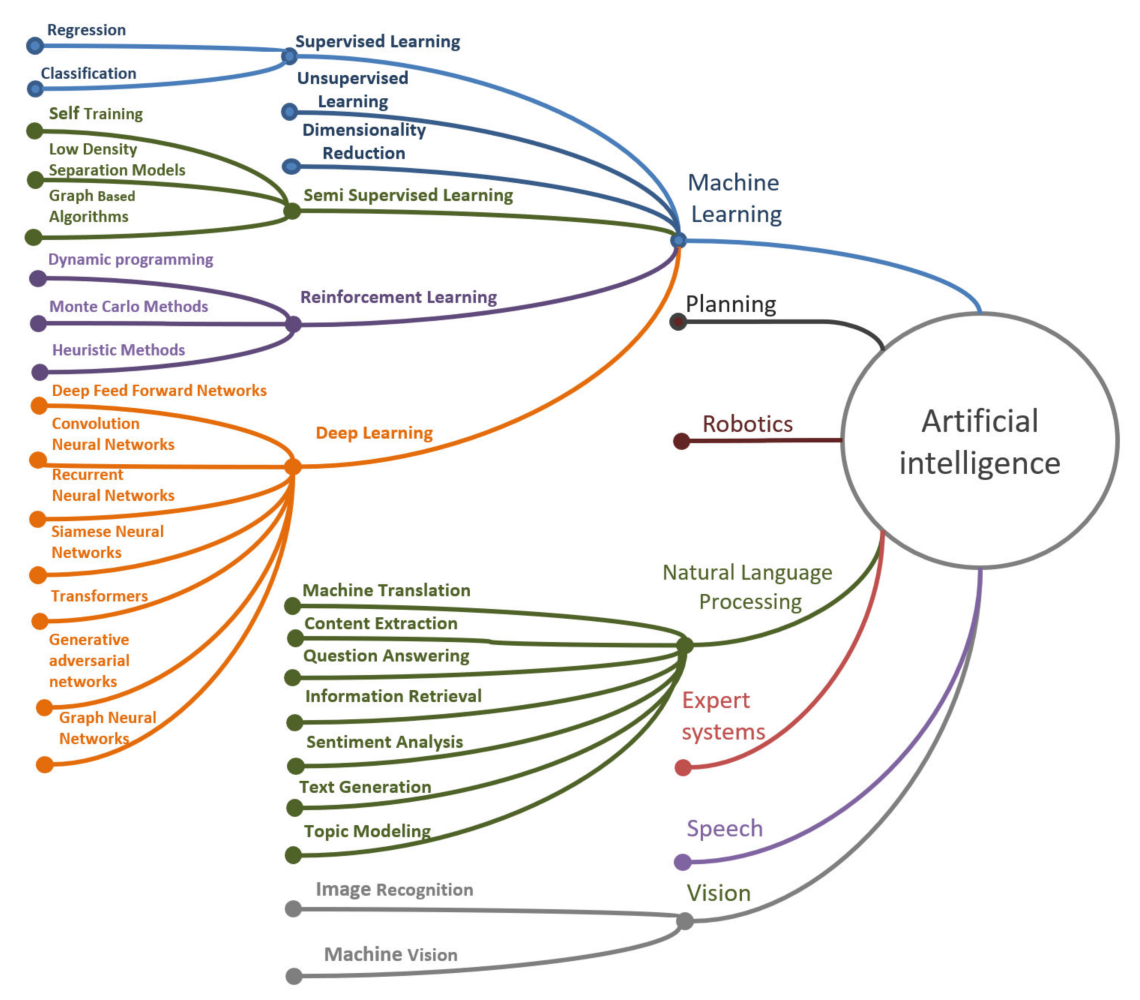
\includegraphics[width=0.9\textwidth]{sectionsAI.png}
	\caption{Campos de la Inteligencia Artificial \cite{artInt}.}
	\label{fig:imagen23}
\end{figure}

El Aprendizaje Automático (ML), por otra parte, es un campo de la IA que está centrado en el desarrollo de esos algoritmos que les permiten aprender y hacer predicciones a partir de los datos o problemas. Es definido como “capacidad de las máquinas para aprender sin ser programadas específicamente” \cite{deepLearning}. En la práctica, se puede definir como la construcción de modelos matemáticos mediante unos datos de muestra, y realizar con esos modelos predicciones o tomar decisiones sobre datos nuevos. 
\cite{deepLearning}

Los métodos de ML más comunes que se utilizan para aprender y realizar predicciones son los siguientes 
\cite{deepLearning} \cite{artInt}:

\begin{itemize}

    \item \textbf{Aprendizaje Supervisado (SL):} método en el que se utilizan datos etiquetados para el entrenamiento del modelo. Esto quiere decir que para cada dato de entrada existe una salida final que es conocida, y el objetivo del modelo es aprender a unir cada entrada con su salida. Tras tener el modelo entrenado, este será capaz de predecir las salidas no conocidas de nuevas entradas.
    \item \textbf{Aprendizaje No Supervisado (UL):} método en el que se utilizan datos no etiquetados para el entrenamiento del modelo. En este caso, el modelo pretende encontrar patrones ocultos o estructuras en los datos de entrada sin conocer la salida.
    \item \textbf{Aprendizaje Semi-Supervisado (SSL):} método en el que se utiliza una combinación de datos etiquetados y no etiquetados para el entrenamiento del modelo. Este método es útil en caso de que la obtención de los datos etiquetados sea costosa.
    \item \textbf{Aprendizaje por refuerzo (RL):} método en el que se entrena un agente, que interactúa con el entorno realizando determinadas acciones y obteniendo recompensas o penalizaciones dependiendo del resultado de la acción, y aprende con el objetivo de maximizar la recompensa acumulada. Es útil en campos como la robótica, los juegos o la navegación autónoma.
    \item \textbf{Aprendizaje Profundo (DL):} conjunto de métodos más complejos que utilizan redes de neuronas artificiales con múltiples capas ocultas para aprender patrones en un conjunto de datos muy grande. Las arquitecturas de DL más conocidas son redes neuronales recurrentes (RNN) y redes neuronales convolucionales (CNN).

\end{itemize}

\begin{figure}[h]
	\centering
	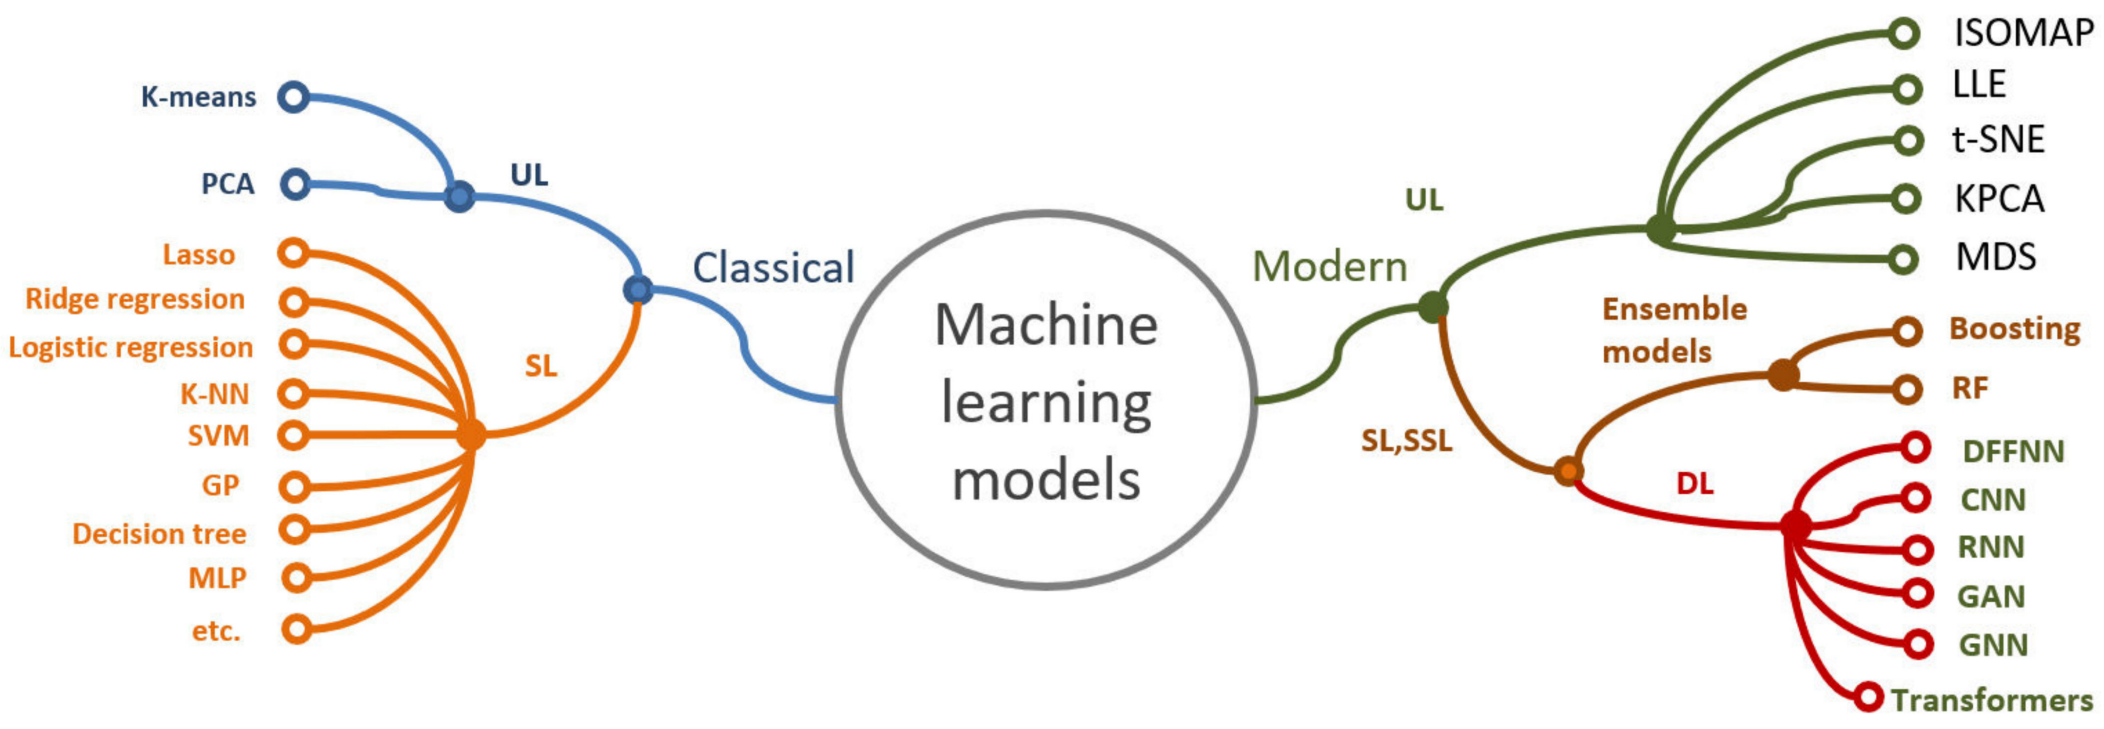
\includegraphics[width=0.9\textwidth]{modelsML.png}
	\caption{Modelos de Aprendizaje Automático \cite{artInt}.}
	\label{fig:imagen24}
\end{figure}

\subsection{Redes Neuronales}

Una red de neuronas artificial (ANN), o simplemente red de neuronas, es un sistema basado en múltiples nodos llamados neuronas, distribuidas en varias capas. Las capas principales de una red de neuronas son la capa de entrada que recibe los datos, las capas ocultas que procesan los datos, y la capa de salida que devuelve los resultados. 
\cite{annReview}

Cada neurona de una capa recibe entradas, procesa esas entradas y devuelve una salida que es enviada a la capa siguiente. El proceso de un dato en una neurona se realiza a través de una función de activación, función que introduce características no lineales en la red para que pueda aprender relaciones complejas entre el dato de entrada y salida.

\begin{figure}[h]
	\centering
	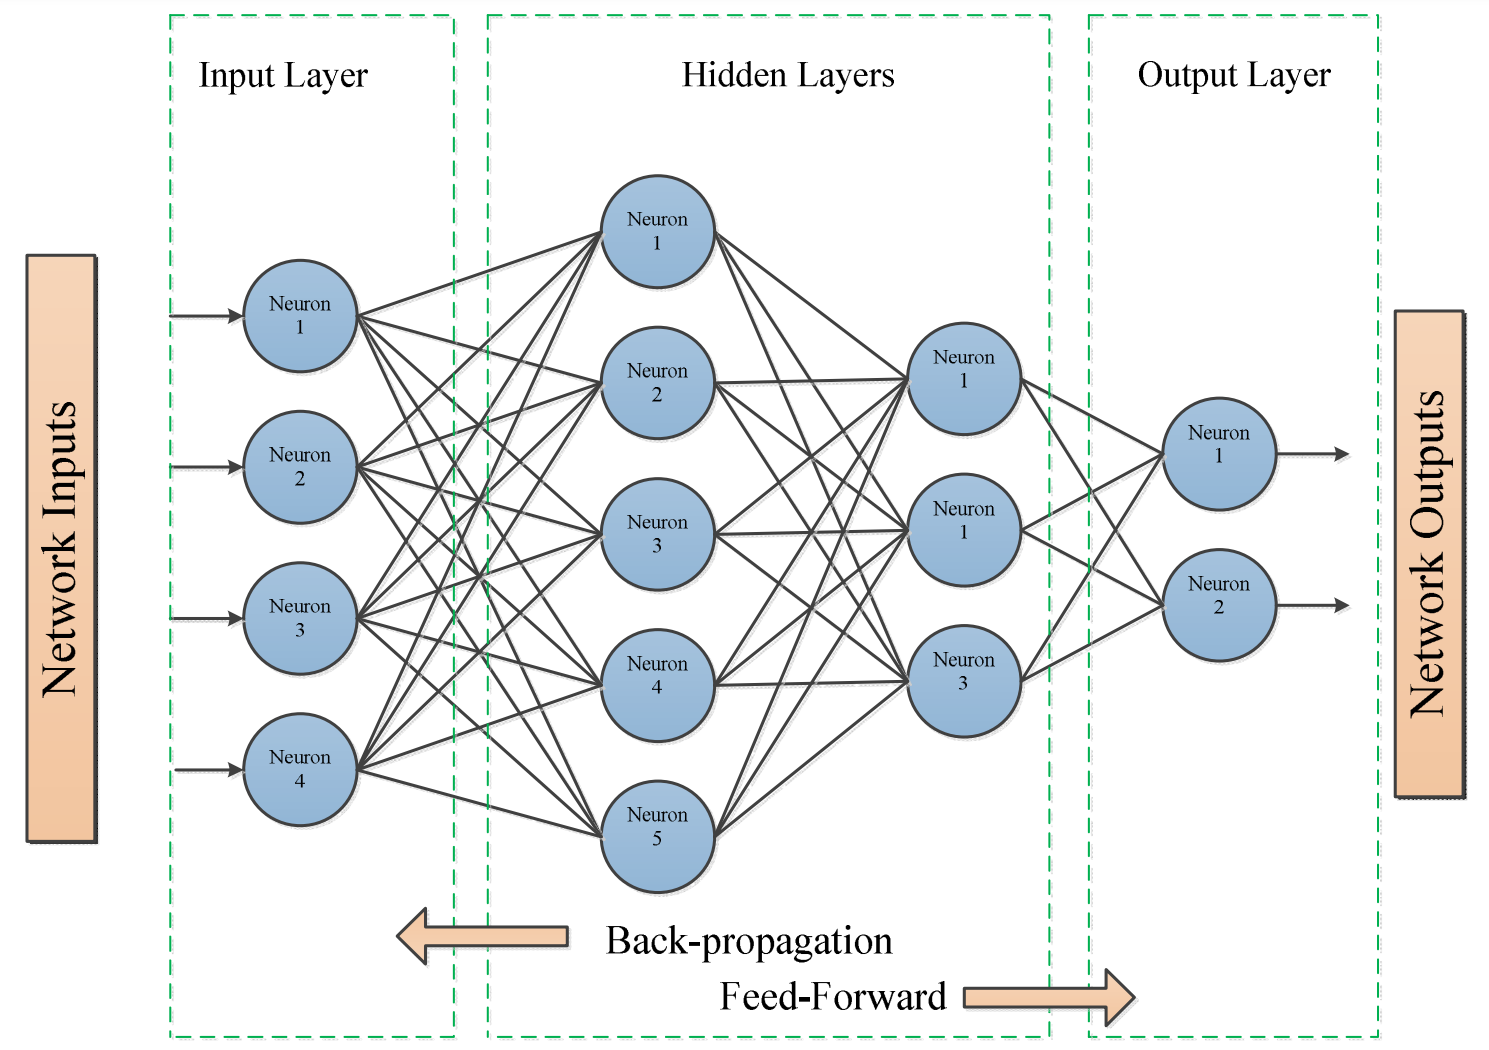
\includegraphics[width=0.7\textwidth]{annStructure.png}
	\caption{Artificial Neural Network basic architecture \cite{annReview}.}
	\label{fig:imagen25}
\end{figure}

\subsubsection{Redes Neuronales Recurrentes (RNN)}

Las redes de neuronas recurrentes (RNN) son un tipo de red neuronal que destacan por tener conexiones en forma de ciclos en la red, permitiéndoles mantener una “memoria” de los estados anteriores, por lo que son eficaces con el tratamiento de tareas donde tiene importancia el contexto temporal. 
\cite{artInt} \cite{annReview}

Las RNN procesan los datos de manera secuencial: en cada estado de procesamiento, se toma un valor de entrada y su estado anterior, y a partir de ambas genera una salida y actualiza su estado. Este modo de procesamiento en forma de ciclo es lo que permite a la red mantener la “memoria” de la información a lo largo de todo el proceso, y lo que es relevante para tareas como el procesamiento del lenguaje natural (NLP), donde la comprensión de una palabra depende del contexto anterior.

\begin{figure}[H]
	\centering
	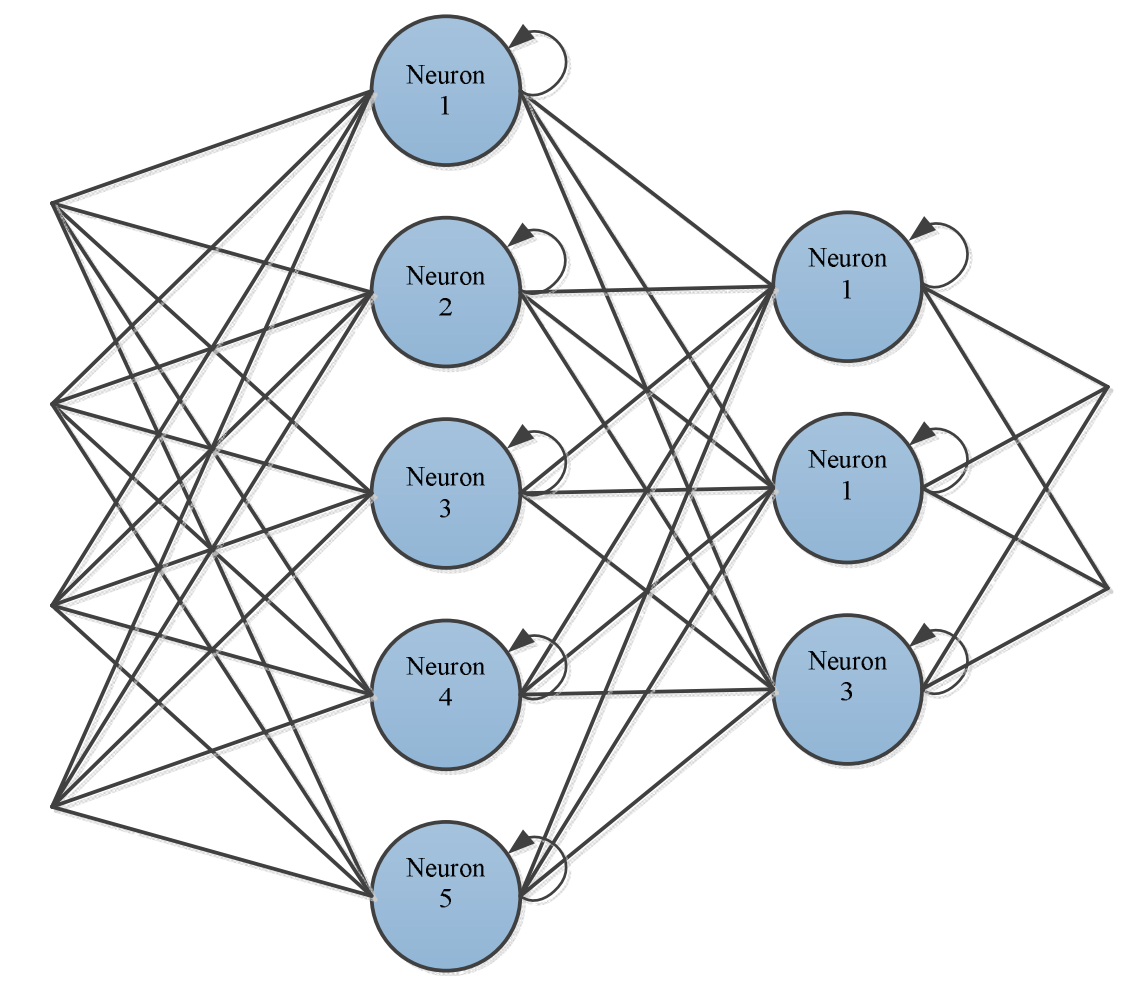
\includegraphics[width=0.5\textwidth]{rnnStructure.png}
	\caption{Recurrent Neural Network basic architecture \cite{annReview}.}
	\label{fig:imagen26}
\end{figure}

\subsubsection{Redes Neuronales Convolucionales (CNN)}

Las  redes de neuronas convolucionales (CNN) son un tipo de red neuronal que destacan por poder procesar y analizar datos que tengan una estructura de cuadrícula, como por ejemplo las imágenes. 
\cite{artInt} \cite{annReview}

Una CNN está compuesta por varias capas de distintos tipos que transforman la entrada recibida de una manera específica:

\begin{itemize}

    \item \textbf{Capa convolucional:} capa que aplica filtros o núcleos a los datos de entrada, siendo el filtro una matriz pequeña que se desliza sobre el dato, y realiza una convolución sobre los datos para obtener un mapa de características. Estas características son las que permiten a la red detectar los patrones en la imagen, como bordes o texturas.
    \item \textbf{Capa de pooling o subsampling:} capa que aplica una reducción de dimensionalidad sobre el mapa de características, generalmente siendo una operación de max-pooling tomando el valor máximo de cada región. Esta capa sirve para reducir la cantidad de parámetros y controlar el sobreajuste.
    \item \textbf{Capas completamente conectadas:} capas que se sitúan al final de la red, y sirven para procesar las características obtenidas de las capas anteriores y realizar una clasificación final. Cada neurona de esta capa se conecta a todas las neuronas de la capa anterior.

\end{itemize}

\begin{figure}[H]
	\centering
	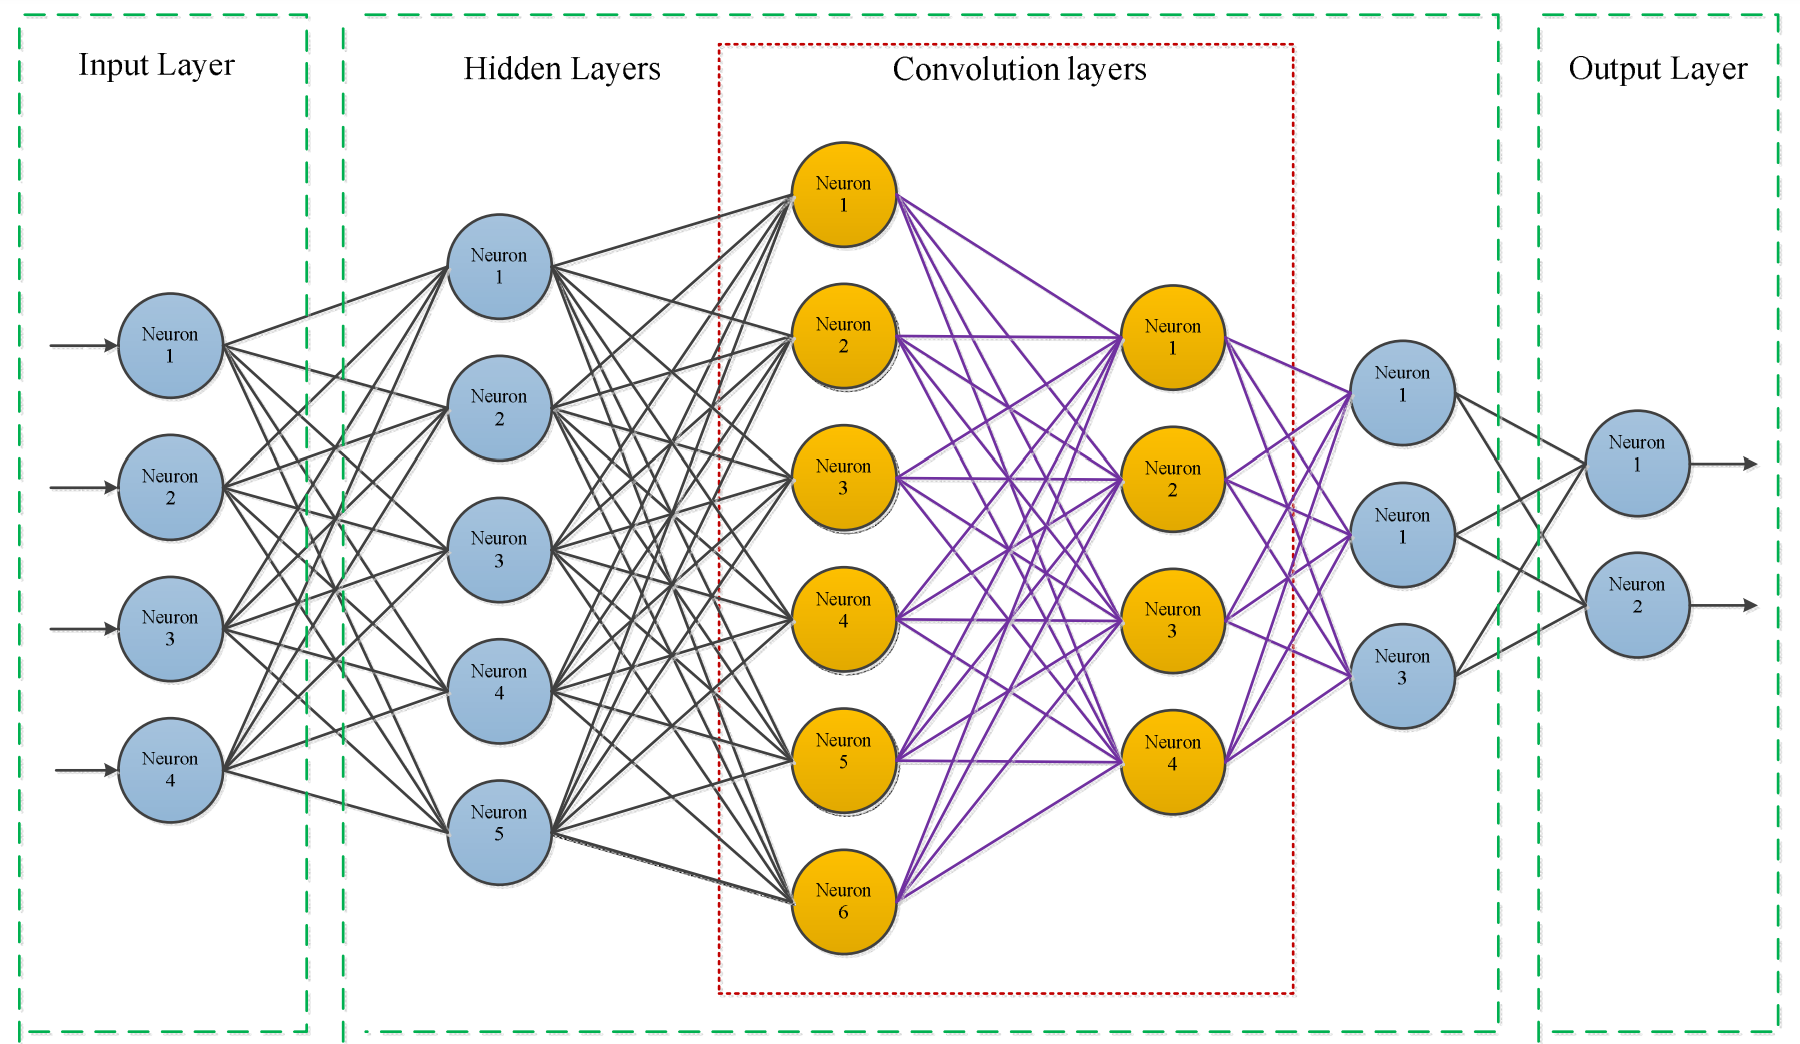
\includegraphics[width=0.9\textwidth]{cnnStructure.png}
	\caption{Convolutional Neural Network basic architecture \cite{annReview}.}
	\label{fig:imagen27}
\end{figure}

\begin{figure}[H]
	\centering
	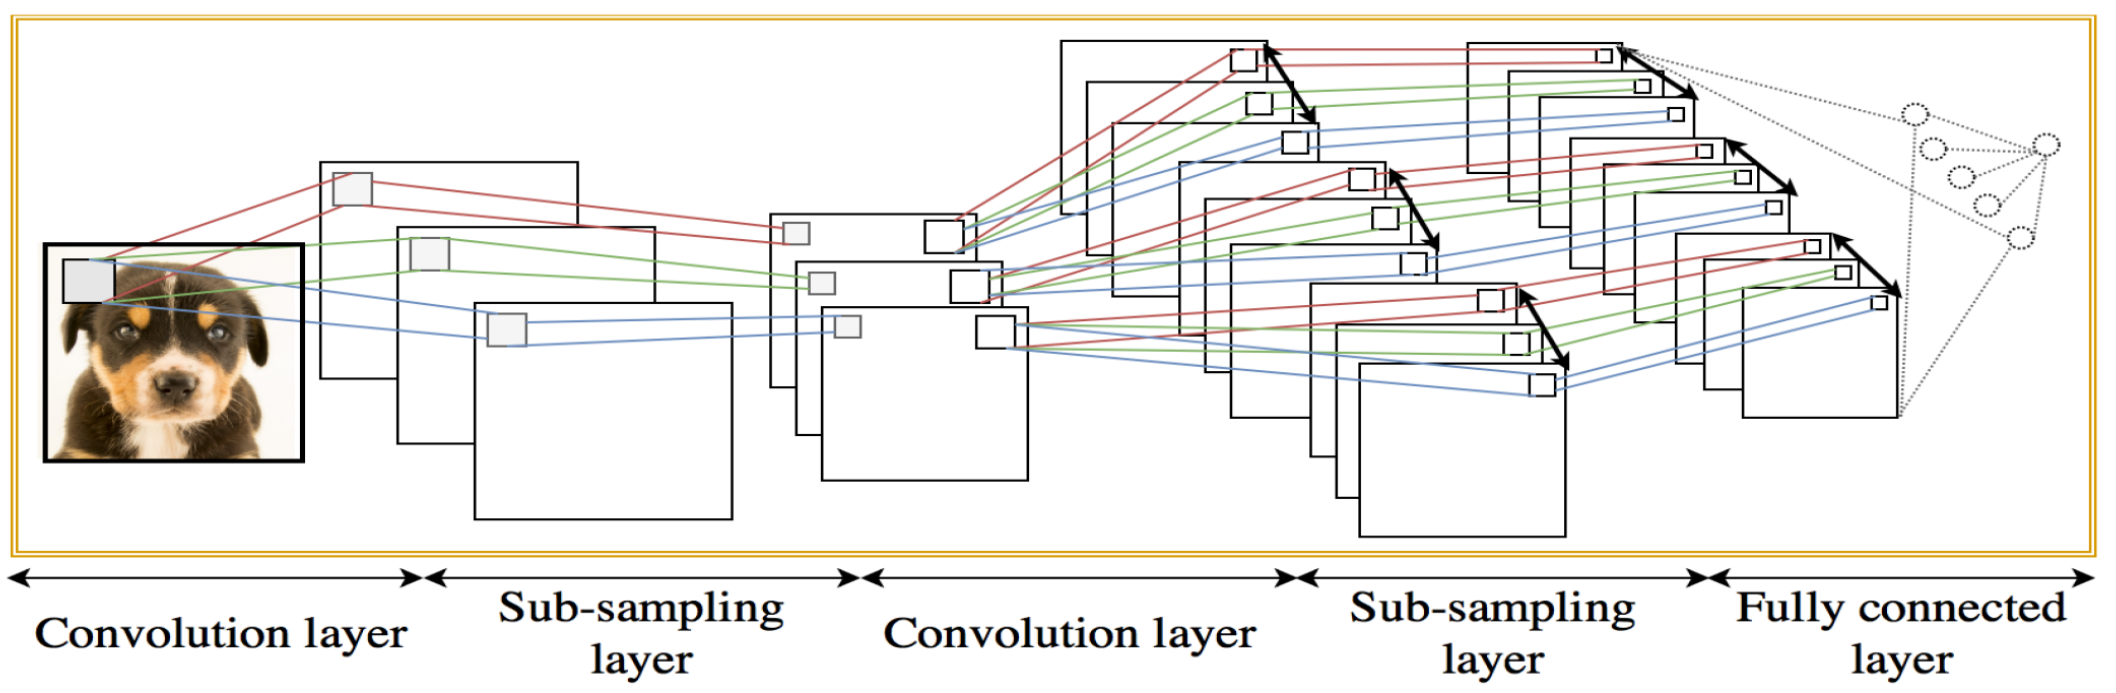
\includegraphics[width=0.9\textwidth]{basicCnn.png}
	\caption{Convolutional Neural Network layers visualization \cite{deepImages}.}
	\label{fig:imagen28}
\end{figure}

\section{Trabajos Relacionados}

El reconocimiento de emociones ya sea de los ocupantes o del conductor en un vehículo es un área de desarrollo fundamental para la industria automotriz. Una capacidad para identificar y responder eficaz puede mejorar considerablemente la seguridad o la experiencia de usuario de los ocupantes del vehículo. Al ser un área de investigación que ha ido avanzado a lo largo de los años, se han realizado muchos estudios destacados, llegando al estado actual con sistemas tecnológicos cada vez más sofisticados.

Un proyecto interesante y reciente es “Drivers’ Comprehensive Emotion Recognition Based on HAM” \cite{rw1} realizado en 2023, basado en mejorar la precisión de modelos de aprendizaje profundo para reconocer emociones, en este caso del conductor, utilizando señales audiovisuales. La metodología utilizada es una combinación híbrida de diferentes redes neuronales, y un entrenamiento y validación con distintos conjuntos de datos, y lograron una precisión del 79.60\% en el conjunto de datos FER2013 superando a otros modelos ya existentes.

Otro proyecto destacado es “AI-Powered In-Vehicle Passenger Monitoring Using Low-Cost mm-Wave Radar” \cite{rw2} publicado en 2021, en el que se desarrolla un sistema de detección y monitoreo de los pasajeros de un vehículo. Concretamente, trata de identificar los asientos ocupados y contar el número de pasajeros que hay mediante un radar de onda milimétrica generando mapas de calor, y procesando la información con algoritmos de aprendizaje automático. En comparación con los sistemas tradicionales, este sistema permite detectar pasajeros con más precisión, como por ejemplo al detectar múltiples pasajeros en asientos adyacentes, además de ser una solución económica con el uso de radares de bajo costo.

En cuanto a proyectos en relación a la experiencia de usuario, un proyecto destacado es “Mobility Prediction-Based Optimisation and Encryption of Passenger Traffic-Flows Using Machine Learning” \cite{rw3} publicado en 2020. Este proyecto se centra en desarrollar un modelo predictivo de aprendizaje automático para mejorar el rendimiento de infraestructuras ferroviarias, en este caso del metro de Londres, abordando problemas como la congestión, los accidentes, la sobrecarga de vagones o el mantenimiento. Utilizan sensores de identificación por radiofrecuencia (RFID) que registran los datos de pasajeros en tiempo real mediante tecnología 5G, y con un modelo de redes neuronales artificiales predicen los patrones de flujo de los pasajeros. Además todos los datos enviados en tiempo real son encriptados lo que asegura su seguridad y privacidad. Realizaron simulaciones con datos reales del metro de Londres y el modelo alcanzó una precisión del 91.17\% en la predicción del flujo de movilidad de los pasajeros.

Otro ejemplo de proyecto es “Estimating passenger experience from vehicle data: Preconditions for using machine learning” \cite{rw4} publicado en 2020. Este artículo se centra en evaluar métodos de aprendizaje automático para estimar de forma automática la experiencia de los pasajeros en los autobuses eléctricos, utilizando datos obtenidos con sensores en el autobús y encuestas a los pasajeros sobre la experiencia del viaje. Las implicaciones de este estudio puede ser interesante para los fabricantes de vehículos, ya que podrían mejorar su diseño y desarrollo, o para los operadores de los transportes públicos, ya que podrían mejorar la formación de conductores o la planificación de rutas en función de la satisfacción del pasajero. 

Otro proyecto, también relacionado a mejorar la experiencia de usuario sobre el uso de autobuses como medio de transporte público, es “A Real-Time Machine Learning-Based Public Transport Bus-Passenger Information System” \cite{rw5} publicado en 2021. El objetivo de este estudio es desarrollar un sistema de información en tiempo real que muestra la ubicación de los autobuses para mejorar su puntualidad y confiabilidad, y optimizar la asignación de recursos mediante técnicas de machine learning, usando datos diarios para predecir demandas de pasajeros en diferentes rutas. Esto servirá para estimar de una manera más exacta el tiempo de llegada de un autobús y por lo tanto optimizar tiempo, además de asignar de una manera más eficiente autobuses a las diferentes rutas que lo necesiten.

\section{Conclusiones y Análisis de Resultados}

Tras haber realizado un análisis e investigación del Estado del Arte y los proyectos realizados en relación al tema, se ha podido observar que en la evolución del automóvil el factor de la seguridad es un papel muy importante e innovador, sobre todo en las tecnologías ADAS. Esto es debido sobre todo a los avances tecnológicos de los sensores, las mejoras en las capacidades de cómputo y el desarrollo de algoritmos más avanzados de IA, todo esto de relación muy importante si en un futuro se quiere transicionar de vehículos tradicionales a vehículos autónomos.

La mayoría de los sistemas ADAS actualmente están diseñados para asistir al conductor, mientras que no hay muchos que sean enfocados a los pasajeros. Pero la experiencia del usuario, ya sea centrada en la seguridad como en la comodidad, debería tener igual importancia, y más en los vehículos autónomos donde la presencia del conductor será cada vez menor.

Tras obtener estas conclusiones del análisis, con este proyecto se pretende proponer un sistema, cuyo diseño se centra en mejorar la experiencia de usuario de los ocupantes de un vehículo, y que funcione a partir de análisis en tiempo real de sus emociones y reaccionar de una manera u otra interactuando con las funcionalidades de los vehículos, como son el sonido de la música o radio, el aire acondicionado, la comodidad de los asientos, o integrarse en sistemas ADAS que sirvan para mejorar la experiencia de los ocupantes.

\chapter{Diseño del sistema}



\chapter{Implementación y resultados}



\chapter{Marco regulador}



\chapter{Entorno socio-económico}

\section{Gestión del proyecto}



\section{Impacto socio-económico}



\chapter{Conclusiones y trabajos futuros}


%----------
%	BIBLIOGRAFÍA
%----------	

%\nocite{*} % Si quieres que aparezcan en la bibliografía todos los documentos que la componen (también los que no estén citados en el texto) descomenta está línea

\clearpage
\addcontentsline{toc}{chapter}{Bibliografía}
\setquotestyle[english]{british} % Cambiamos el tipo de cita porque en el estilo IEEE se usan las comillas inglesas.
\printbibliography



%----------
%	ANEXOS
%----------	

% Si tu trabajo incluye anexos, puedes descomentar las siguientes líneas
%\chapter* {Anexo x}
%\pagenumbering{gobble} % Las páginas de los anexos no se numeran



\end{document}